\documentclass[12pt]{article}
\usepackage[left=3.5cm,right=2cm,top=2.5cm,bottom=2.5cm]{geometry}
\usepackage[T1]{fontenc}
\usepackage[utf8]{inputenc}
\usepackage{tgpagella}
\usepackage{enumerate}
\usepackage{url}
\usepackage{multirow}
\usepackage{longtable}
\usepackage{polski}
\usepackage{graphicx}
\usepackage{float}
\usepackage{color}
\usepackage{amsmath}
\usepackage{longtable}
\usepackage{tabularx}
\usepackage{ltablex,booktabs}
\usepackage{amssymb}
\usepackage{rotating}
\usepackage{subfigure}
\usepackage{float}
\usepackage{tabu}
\usepackage{caption}
\usepackage{footnote}
\usepackage{xspace}
\usepackage{mathpazo}
\usepackage[table]{xcolor}
\usepackage[justification=centering]{caption}
\graphicspath{ {images/} }

\pagestyle{empty}

\title{\LARGE{Uniwersytet Wrocławski}\\
\Large{Wydział Matematyki i Informatyki}\\
\large{Kierunek: Informatyka}}

\date{}

\begin{document}
\pagestyle{empty}

\begin{titlepage}
\maketitle
\thispagestyle{empty}


\begin{center}
\author{\LARGE{Adrian Mularczyk}}
\vspace{30pt}

\huge{\textbf{Stworzenie wydajnego wzorca wstrzykiwania zależności dla złożonych grafów zależności}}
\vspace{50pt}
\end{center}

\begin{flushright}
\large{Praca wykonana pod kierunkiem}
\large{dr. Wiktora Zychli}
\end{flushright}

\vfill
\begin{center}
\begin{large}
Wrocław, 2016
\end{large}
\end{center}
\end{titlepage}


\setlength{\parindent}{0pt}	%usunięcie wcięć
\setlength{\parskip}{1.5ex} 
\renewcommand*{\figurename}{Rys.}
\renewcommand*{\tablename}{Tab.} 
\renewcommand{\captionsize}{\small}

\setlength{\intextsep}{0pt}


\newpage
\setcounter{page}{2}
\pagestyle{plain}
\textcolor{white}{  }
\begin{center}
\vspace{50pt}
\textbf{\emph{Oświadczenie opiekuna pracy}}\\
\end{center}
Oświadczam, że niniejsza praca została przygotowana pod moim kierownictwem i stwierdzam, że spełnia ona warunki do przedstawienia jej w postępowaniu o nadanie tytułu naukowego.\\

\vspace{54pt}

\begin{tabular}{lccccccccr}
Data................... & & & & & & & & & Podpis opiekuna pracy ..................................... \\
\end{tabular}


\vspace{150pt}

\begin{center}
\textbf{\emph{Oświadczenie autora pracy}}\\
\end{center}
Oświadczam, że niniejsza praca dyplomowa została napisana przeze mnie samodzielnie i nie zawiera treści uzyskanych w sposób niezgodny z obowiązującymi przepisami ani też nie była wcześniej przedmiotem procedur związanych z uzyskaniem tytułu zawodowego w wyższej uczelni.\\

\vspace{54pt}

\begin{tabular}{lccccccccr}
Data................... & & & & & & & & & Podpis autora pracy ..................................... \\
\end{tabular}


\clearpage
\begin{center}
\textbf{Streszczenie}\\
\vspace{16pt}
\textbf{Stworzenie wydajnego wzorca wstrzykiwania zależności dla złożonych grafów zależności}
\end{center}
Wstrzykiwanie zależności jest to zbiór zasad projektowania oprogramowania, które umożliwiają luźne powiązania. Dzięki temu kod jest rozszerzalny i łatwiejszy w utrzymaniu. Celem tej pracy było stworzenie takiej realizacji, która będzie sprawdzała się dla złożonych grafów zależności. Aplikacja została napisana w środowisku .NET z wykorzystaniem przestrzeni nazw Reflecion.Emit oraz jest w pełni przetestowana. W pracy zaproponowano dwa równorzędne, niezależne podejścia, oba porównano pod kątem wydajnościowym. Porównanie obejmuje również 5 najbardziej popularnych i 4 najszybsze rozwiązania. Końcowe wyniki wykazały, że z obecnie dostępnych rozwiązań na rynku, zaprezentowane w niniejszej pracy radzi sobie najlepiej.

\clearpage
\begin{center}
\textbf{Abstract}\\
\vspace{16pt}
\textbf{Creating an efficient dependency injection pattern for complex dependency graphs}
\end{center}
Injection Dependency is a set of software design principles that allow for loose binding. This makes the code more extensible and easier to maintain. The purpose of this work was to create such an implementation that would work efficiently for complex dependency graphs. The application was written in a .NET environment using the Reflecion.Emit namespace and is fully tested. The paper proposes two equivalent, independent approaches which are compared for performance. The comparison also includes the 5 most popular and 4 fastest solutions. The final results show that from solutions available nowadays on the market, the best solutions are these presented in this paper.


\clearpage
\tableofcontents


\clearpage
\section{Wstęp}
\subsection{Cel pracy}
Wstrzykiwanie zależności jest wzorcem projektowym, który pozwala na tworzenie kodu o luźniejszych powiązaniach, łatwiejszego w testowaniu i modyfikacji. Najbardziej popularnymi implementacjami tego wzorca na platformie .NET są Unity i Ninject. Niestety większość rozwiązań skupia się na zapewnieniu jak największej liczby funkcjonalności, co ma negatywne skutki dla wydajności. O ile przy małej liczbie zależności te czasy nie są zbyt duże, to wraz ze wzrostem zależności wydajność zauważalnie spada.\\
\\
Celem niniejszej pracy magisterskiej jest stworzenie takiej implementacji tego wzorca, która będzie wydajna dla złożonych grafów zależności, ale również będzie dostarczać niezbędnej funkcjonalności. Do tego celu zostaną wykorzystane mechanizmy z przestrzeni nazw Reflection.Emit. W tej pracy zostaną przedstawione dwa rozwiązania tego problemu.

\subsection{Układ pracy}
Poza wstępem i podsumowaniem praca składa się jeszcze z czterech rozdziałów. Pierwszy z nich opisuje idee stojące za wstrzykiwaniem zależności. W kolejnym znajduje się opis teoretyczny tego czym jest wstrzykiwanie zależności. Następny rozdział został poświęcony mojej implementacji tego wzorca. Ostatni z rozdziałów skupia się na testach wydajnościowych, w których są porównywane rozwiązanie przedstawione w tej pracy, z kilkoma najbardziej popularnym i kilkoma najwydajniejszymi rozwiązaniami.



\clearpage
\section{Odwrócenie zależności}
\subsection{SOLID}
Na przestrzeni lat powstało bardzo dużo projektów. Część z nich była łatwiejsza w utrzymaniu, część trudniejsza. Analiza tych projektów pozwoliła zauważyć, że są pewne zasady, które powodują, że projekty rozwija się łatwiej. Te zasady zostały połączone w zbiory zasad. Najbardziej popularnych i powszechnie stosowanym zbiorem zasad jest SOLID \cite{SOLID}:
\begin{itemize}
	\item S (Single responsibility principle) - Klasa powinna mieć tylko jedną odpowiedzialność (nigdy nie powinien istnieć więcej niż jeden powód do modyfikacji klasy).
	\item O (Open/closed principle) - Klasy powinny być otwarte na rozszerzenia i zamknięte na modyfikacje.
	\item L (Liskov substitution principle) - Funkcje które używają klas bazowych, muszą być w stanie używać również obiektów klas dziedziczących po klasach bazowych, bez dokładnej znajomości tych obiektów.
	\item I (Interface segregation principle) - Wiele dedykowanych interfejsów jest lepsze niż jeden ogólny.
	\item D (Dependency inversion principle) - Wysokopoziomowe moduły nie powinny zależeć od modułów niskopoziomowych - zależności między nimi powinny wynikać z abstrakcji.
\end{itemize}
Niniejsza praca w dużej mierze skupia się na rozwiązaniu dla zasady D - Dependency inversion principle. 

\subsubsection{Przykład dla zasady D}
Rysynek \ref{fig:Solid_without} przedstawia przykład przed zastosowaniem zasady D.\\
\begin{figure}[H]
	\begin{center}
  		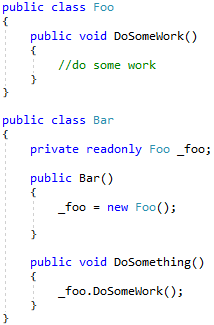
\includegraphics{Solid_without.png}
  		\caption{Przykładowa klasa bez zasady D}
  		\label{fig:Solid_without}
	\end{center}
\end{figure}
Rysunek \ref{fig:Solid_with} przedstawia przykład po zastosowaniu zasady D.\\
\begin{figure}[H]
	\begin{center}
  		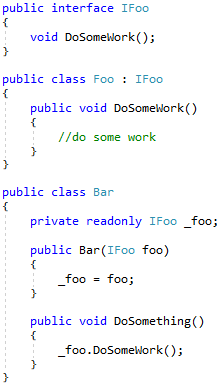
\includegraphics{Solid_with.png}
  		\caption{Przykładowa klasa z zasadą D}
  		\label{fig:Solid_with}
	\end{center}
\end{figure}
Łatwo zauważyć, że teraz klasy Bar nie interesuje implementacja klasy Foo. Spodziewa się jedynie, że dostanie implementację interfejsu IFoo, który dostarcza metody DoSomeWork. Dzięki takiemu podejściu w łatwy sposób można podmienić implementację interfejsu IFoo w klasie Bar. Zatem tworząc ciało metody DoSomething w klasie Bar nie przejmujemy się implementacją metody DoSomeWork, tylko rozważamy jej "kontrakt", zobowiązanie do realizacji założonej funkcjonalności.\\
\\
Kolejną zaletą takiego podejścia jest to, że teraz w łatwy sposób można przetestować metodę DoSomething - można stworzyć przykładową implementację interfejsu IFoo lub użyć tzw. obiektu zastępczego (ang. mock).


\subsection{Kontenery wstrzykiwania zależności}
Aby łatwiej zastosować zasadę D można wesprzeć się tzw. kontenerem wstrzykiwania zależności (ang. Dependency Injection Container) - obiektem, który przechowuje mapę, w której abstrakcje (interfejsy, klasy abstrakcyjne) mają przyporządkowane implementacje (klasy implementujące interfejsy lub dziedziczące z klas abstrakcyjnych).\\
\\
Kontenery dostarczają nam kilku funkcjonalności. Jedną z nich jest oczywiście możliwość zdefiniowania tego jakiej konkretnej klasy instancję należy zwrócić w miejsce konkretnego interfejsu. Drugą, również ważną funkcjonalnością jest tworzenie, na podstawie przechowywanego mapowania, instancji obiektów konkretnej klasy lub implementujących określony interfejs. Niektóre kontenery dostarczają również mechanizmy pozwalające rozszerzyć tworzenie nowych instancji o elementy programowania aspektowego.



\clearpage
\section{Wstrzykiwanie zależności}
\subsection{Wstęp}
Wstrzykiwanie zależności jest niczym więcej niż techniką, która umożliwia luźne powiązania, a luźne powiązania sprawiają, że kod jest rozszerzalny i łatwy w utrzymaniu.\cite{dependency_injection}\\
Wstrzykiwanie zależności może odbywać się na 3 sposoby:
\begin{itemize}
	\item wstrzykiwanie przez konstruktor
	\item wstrzykiwanie przez metodę
	\item wstrzykiwanie przez właściwość
\end{itemize}

\subsubsection{Wstrzykiwanie przez konstruktor}
Jest to główny i najbardziej popularny sposób wstrzykiwania zależności. Niektóre klasy mają więcej niż jeden konstruktor i atrybut "DependencyConstructor" przydaje się wtedy do oznaczenia, który z nich ma zostać wybrany przy tworzeniu nowego obiektu. Przykład klasy z atrybutem DependencyConstructor przedstawia Rys. \ref{fig:DependencyConstructor}.\\ \\
\begin{figure}[H]
	\begin{center}
  		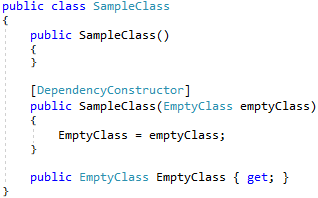
\includegraphics{DependencyConstructor.png}
  		\caption{Przykładowa klasa z atrybutem DependencyConstructor}
  		\label{fig:DependencyConstructor}
	\end{center}
\end{figure}

\subsubsection{Wstrzykiwanie przez metodę}
To wstrzykiwanie z reguły odbywa się albo poprzez oznaczenie metody przez którą chcemy wstrzyknąć zależności odpowiednim atrybutem, albo przez wskazanie odpowiedniej metody podczas rejestracji. Przykład klasy z oznaczeniem metody odpowiednim atrybutem przedstawia Rys. \ref{fig:DependencyMethod}.
\begin{figure}[H]
	\begin{center}
  		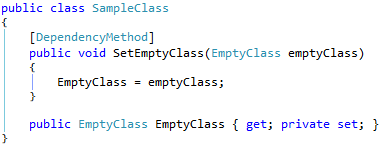
\includegraphics{DependencyMethod.png}
  		\caption{Przykładowa klasa z atrybutem DependencyMethod}
  		\label{fig:DependencyMethod}
	\end{center}
\end{figure}

\subsubsection{Wstrzykiwanie przez właściwość}
Tutaj podobnie jak dla wstrzykiwania przez metodę to wstrzykiwanie z reguły odbywa się albo poprzez oznaczenie właściwości przez którą chcemy wstrzyknąć zależności odpowiednim atrybutem, albo przy rejestracji danej klasy definiujemy przez jakie właściwości chcemy wstrzyknąć zależności. Przykład klasy z oznaczeniem właściwości odpowiednim atrybutem przedstawia Rys. \ref{fig:DependencyProperty}.\\ \\
\begin{figure}[H]
	\begin{center}
  		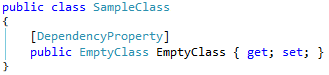
\includegraphics{DependencyProperty.png}
  		\caption{Przykładowa klasa z atrybutem DependencyProperty}
  		\label{fig:DependencyProperty}
	\end{center}
\end{figure}


\subsection{Implementacje przemysłowe}
Na rynku jest wiele implementacji wstrzykiwania zależności. Przedstawię tutaj kilka najbardziej popularnych (według ilości pobrań z NuGet) oraz kilka najszybszych (według rankingu na stronie: http://www.palmmedia.de/Blog/2011/8/30/ioc-container-benchmark-performance-comparison). Dane pochodzą z dnia 21-02-2017. W nawiasie znajduje się wersja implementacji, która została użyta w testach (najnowsza na ten dzień).\\
\\
Najbardziej popularne:
\begin{itemize}
	\item Unity (4.0.1) - ponad 5.2 mln pobrań
	\item NInject (3.2.2) - ponad 4.0 mln pobrań
	\item Autofac (4.3.0) - ponad 3.7 mln pobrań
	\item StructureMap (4.4.3) - ponad 1.6 mln pobrań
	\item Windsor (3.4.0) - ponad 1.4 mln pobrań
\end{itemize}
Najszybsze:
\begin{itemize}
	\item Grace (5.1.0)
	\item DryIoc (2.10.1)
	\item LightInject (5.0.1)
	\item SimpleInjector (3.3.2)
\end{itemize}



\clearpage
\section{Implementacja}
Kod źródłowy programu jest dostępnym w repozytorium pod adresem:\\
\url{https://github.com/amularczyk/NiquIoC}\\
Znajduje się tam również kod programu, który posłużył do wykonania testów wydajnościowych, a także ta praca napisana w języku LateX i wszystkie obrazki.

\subsection{Środowisko pracy}
Praca oraz wszystkie testy powstały na komputerze z parametrami:
\begin{itemize}
	\item Intel Core i7-4720HQ (2.60GHz)
	\item 12 GB pamięci RAM
	\item Dysk SSD
\end{itemize}
Narzędzia użyte do stworzenia pracy i testów:
\begin{itemize}
	\item System operacyjny Windows 10 Pro
	\item .Net Framework w wersji 4.6.1
	\item Visual Studio 2017 Comunnity
	\item MSTest
	\item ReSharper
	\item dotCover
	\item Dia
\end{itemize}


\subsection{Wstęp}
Na początku chciałbym pokrótce opisać dwie rzeczy, które są istotne dla rozwiązania przedstawionego w tej pracy. Pierwszą z nich jest Common Intermediate Language, a drugą przestrzeń nazw Reflection.Emit.

\subsubsection{Common Intermediate Language}
Common Intermediate Language - CIL (w skrócie IL) to język pośredni do którego kod C\# jest kompilowany. Język ten pozwala na komunikację między aplikacjami napisanymi na platformie .NET, a systemem operacyjnym.

\subsubsection{Reflection.Emit}
Przestrzeń nazw Reflection.Emit pozwala w kodzie programu, w sposób dynamiczny, na utworzenie listy operacji w języku IL, a następnie zapamiętaniu ciągu tych operacji jako delegat. Za każdym razem, gdy ten delegat zostanie wywołany, to wykona się ciąg wcześniej zdefiniowanych operacji IL.


\subsection{Opis}
Aplikacja składa się z 1 głównego projektu i 8 projektów na potrzeby testów. Rozwiązanie jest stosunkowo złożone i aby mieć pewność, że działa w pełni dobrze, zostało stworzone  ponad 1250 testów jednostkowych, a pokrycie kodu testami wynosi ponad 97\%.\\

W wykonanej implementacji został stworzony interfejs IConatiner, który składa się z interfejsów zawierających niezbędne operacje, jakie powinny się znaleźć w każdym kontenerze (Rys. \ref{fig:IContainer}).\\ \\
\begin{figure}[H]
	\begin{center}
  		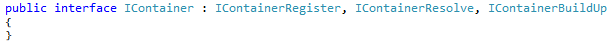
\includegraphics{IContainer.png}
  		\caption{Interfejs IContainer}
  		\label{fig:IContainer}
	\end{center}
\end{figure}
Pierwszy z tych interfejsów to IContainerRegister (Rys. \ref{fig:IContainerRegister}). Zawiera on metody służące do zarejestrowania typów w kontenerze.\\ \\
\begin{figure}[H]
	\begin{center}
  		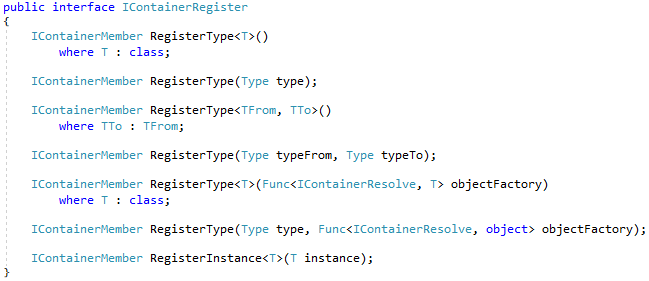
\includegraphics{IContainerRegister.png}
  		\caption{Interfejs IContainerRegister}
  		\label{fig:IContainerRegister}
	\end{center}
\end{figure}
Drugi z nich to IContainerResolve (Rys. \ref{fig:IContainerResolve}). Składa się on z metod odpowiedzialnych za  tworzenie i zwracanie obiektów wcześniej zarejestrowanych typów.\\ \\
\begin{figure}[H]
	\begin{center}
  		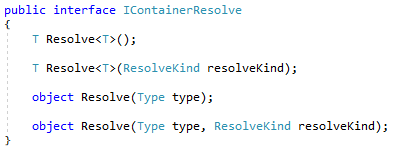
\includegraphics{IContainerResolve.png}
  		\caption{Interfejs IContainerResolve}
  		\label{fig:IContainerResolve}
	\end{center}
\end{figure}
Ostatni z tych interfejsów to IContainerBuildUp (Rys. \ref{fig:IContainerBuildUp}). Jego metody służą do uzupełnienia istniejącej instancji obiektu z wykorzystaniem wstrzykiwania zależności przez metodę i właściwość - są to operacje opcjonalne i nie każde przemysłowe rozwiązanie je zawiera.\\ \\
\begin{figure}[H]
	\begin{center}
  		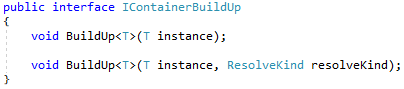
\includegraphics{IContainerBuildUp.png}
  		\caption{Interfejs IContainerBuildUp}
  		\label{fig:IContainerBuildUp}
	\end{center}
\end{figure}
Poniżej znajduje się dokładniejszy opis metod z każdego z powyższych interfejsów.

\subsubsection{Register}
W pierwszej i drugiej metodzie interfejsu IContainerRegister można zarejestrować zwykłe klasy. W trzeciej i czwartej interfejsy oraz klasy, które implementują dany interfejs lub klasy i klasy po nich dziedziczące. W piątej i szóstej metodzie rejestrujemy klasę jako fabrykę obiektów - funkcję, która ma nam zwrócić pożądany obiekt. W siódmej (ostatniej) natomiast możemy zarejestrować konkretną instancję danego typu.\\
\\
W rozwiązaniu przedstawionym w tej pracy każdy typ może być zarejestrowany tylko raz - ponowna rejestracja tego samego typu nadpisuje istniejącą rejestrację.\\
\\
Każda z tych siedmiu metod rejestracji zwraca interfejs IContainerMember (Rys. \ref{fig:IContainerMember}), który umożliwia nam zarejestrowanie danego typu z określonym menadżerem czasu życia (czyli implementacją interfejsu IObjectLifetimeManager - Rys. \ref{fig:IObjectLifetimeManager}). Celem takiego podejścia jest umożliwienie określenia polityki czasu życia dla nowo tworzonych instancji, ponieważ dla różnych przypadków biznesowych możemy potrzebować, aby obiekt danego typu miał konkretny czas życia.\\ \\
\begin{figure}[H]
	\begin{center}
  		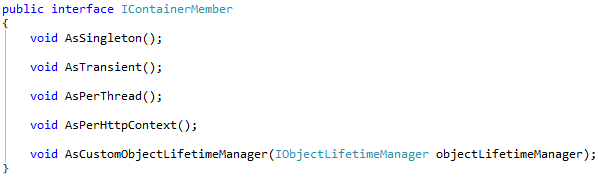
\includegraphics{IContainerMember.png}
  		\caption{Interfejs IContainerMember}
  		\label{fig:IContainerMember}
	\end{center}
\end{figure}
Pierwsze cztery metody interfejsu IContainerMember, to wbudowane implementacje interfejsu IObjectLifetimeManager. Piąta metoda dostarcza możliwość podania przez użytkownika jego własnej implementacji tego interfejsu. Domyślną polityką czasu życia nowo tworzonych instancji jest polityka Transient, czyli zwracanie nowej instancji obiektu za każdym razem, kiedy kontener rozwiązuje zależność.\\
\\
Wyjaśnienie nazw polityk czasu życia:
\begin{itemize}
	\item Singleton - za każdym razem zwracany jest ten sam obiekt
	\item Transient - za każdym razem zwracany jest nowy obiekt
	\item PerThread - wewnątrz danego wątku zwracany jest ten sam obiekt, ale dla innego wątku zwracany jest nowy (inny) obiekt
	\item PerHttpContext - wewnątrz danego żądania Http zwracany jest ten sam obiekt, ale dla innego żądania zwracany jest nowy (inny) obiekt
\end{itemize}

W interfejsie IObjectLifetimeManager właściwość ObjectFactory służy do ustawienia funkcji, która zwraca obiekt. Metoda GetInstance służy do pobrania obiektu.\\
W zależności od implementacji tego interfejsu, to obiekt zwracany z metody GetInstance może być zawsze taki sam, zawsze różny albo taki sam tylko dla określonych sytuacji (np. taki sam dla tego samego wątku albo tego samego żądania http).\\ \\
\begin{figure}[H]
	\begin{center}
  		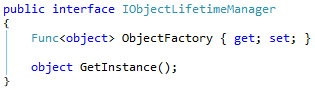
\includegraphics{IObjectLifetimeManager.png}
  		\caption{Interfejs IObjectLifetimeManager}
  		\label{fig:IObjectLifetimeManager}
	\end{center}
\end{figure}

\subsubsection{Resolve}
Metody interfejsu IContainerResolve są głównymi operacjami. Register można nazwać sercem kontenera, a Resolve mózgiem. Każda z metod tego interfejsu odpowiada za stworzenie i zwrócenie obiektu odpowiedniego typu.\\
\\
W niniejszej pracy zaproponowano dwa rozwiązania - PartialEmitFunction i FullEmitFunction (różnice między nimi zostaną opisane w dalszej części pracy), dlatego metody rejestracji jako opcjonalny parametr przyjmuje wartość enumeracji określającej wybraną politykę - ResolveKind (dzięki temu w przyszłości może być ona w łatwy sposób rozszerzona o kolejne rozwiązania). W interfejsie znajdują się również metody, które nie przyjmują tego parametru - zostały one dodane na wypadek, gdy ktoś będzie zawsze korzystał tylko z jednego z rozwiązań (może ustawić je jako domyślne np. w konstruktorze).

\subsubsection{BuildUp}
Interfejs IContainerBuildUp to zwyczajowy, użyteczny dodatek do kontenera - gdy mamy stworzony obiekt, ale nie jest on w pełni uzupełniony, to można go rozbudować (używając metody z odpowiednią wartością enumeracji ResolveKind lub tej z wartością domyślną). Z metodami tego interfejsu są powiązane bezpośrednio dwa pojęcia - wstrzykiwanie przez metodę i wstrzykiwanie przez właściwość. Do tego celu w niniejszym rozwiązaniu utworzono dwa atrybuty:
\begin{itemize}
	\item DependencyMethod (dla metod)
	\item DependencyProperty (dla właściwości)
\end{itemize}
Podczas operacji BuildUp wywoływane są wszystkie metody i uzupełniane są wszystkie właściwości, które mają te atrybuty. Ta operacja jest również wykonywana podczas operacji Resolve.\\
\\
Warto tutaj odnotować, że ze względu na szczegóły implementacyjne tylko jedno z niniejszych rozwiązań wspiera operację BuildUp - jest to rozwiązanie PartialEmitFunction. W rozwiązaniu FullEmitFunction ta funkcjonalność nie została zaimplementowana. Jest to spowodowane skomplikowaniem tego rozwiązania i małą potrzebą biznesową używania tej operacji. Jednakże w przyszłości istnieje możliwość jej dodania.\\

W aplikacji istnieje również atrybut \textbf{DependencyConstructor}. Można go użyć przy definicji konstruktora danej klasy. Obiekt każdej klasy jest tworzony przy użyciu konstruktora. Klasa może mieć kilka konstruktorów. W niniejszym rozwiązaniu utworzono logikę wyboru odpowiedniego konstruktora, przy pomocy którego ma zostać stworzony obiekt. Wygląda ona następująco:
\begin{itemize}
	\item Jeśli jest jeden konstruktor, to go wybierz.
	\item Jeśli jest kilka konstruktorów, to odpowiedni wybierz w poniższej kolejności:
	\begin{enumerate}
		\item Konstruktor z atrybutem DependencyConstructor
		\item Konstruktor z największą liczbą parametrów
	\end{enumerate}
	\item Jeśli jest kilka konstruktorów z atrybutem DependencyConstructor albo nie ma żadnego konstruktora z tym atrybutem i jest kilka z największą liczbą parametrów, to rzuć wyjątek.
\end{itemize}


\subsection{Rozwiązanie}
Utworzenie instancji nowego obiektu zajmuje czas. Gdy graf zależności dla jakiegoś typu jest bardzo rozbudowany, to stworzenie obiektu takiego typu zajmuje dużo czasu. Proces ten można podzielić na trzy etapy:
\begin{itemize}
	\item Uzyskanie informacji jakich typów obiekty są potrzebne do stworzenia danego obiektu.
	\item Stworzenie tych pomocniczych obiektów.
	\item Stworzenie docelowego obiektu.
\end{itemize}
W przypadku rozbudowanych grafów zależności, czasami zdarza się, że niektóre typy się powtarzają. Zatem pewne informacje można uzyskać raz, a następnie je zapamiętać. Aby implementacja wzorca wstrzykiwania zależności działała wydajnie dla złożonych grafów zależności, należy jak najwięcej informacji przechowywać w pamięci podręcznej i należy to robić mądrze.\\
\\
W niniejszej implementacji utworzono dwie strategie, które realizują te założenia. Pierwszy krok jest taki sam dla obu rozwiązań (uzyskanie informacji jakich typów obiekty są potrzebne do stworzenia danego obiektu), natomiast kolejne kroki już się różnią. W pierwszym rozwiązaniu, które nazwano PartialEmitFunction całym proces tworzenia nowego obiektu został rozbity na mniejsze części (docelowy obiekt jest tworzony po kawałku). Każda taka osobna część jest zapisywana w pamięci podręcznej. W drugim rozwiązaniu w pamięci podręcznej jest zapisana tylko jedna operacja. Zawiera ona listę wszystkich kroków, które są niezbędne do stworzenia docelowego obiektu. Więc finalnie docelowy obiekt jest tworzony przy pomocy jednej operacji (kroki drugi i trzeci są połączone). To rozwiązanie nazwano FullEmitFunction.\\
\\
W obu rozwiązaniach do zapamiętania kroków potrzebnych do stworzenia obiektu danego typu wykorzystano operacje z przestrzeni nazw Reflection.Emit.

\subsubsection{Krok pierwszy}
Na początku algorytm znajduje odpowiedni konstruktor, przy pomocy którego ma zostać stworzony nowy obiekt. Jeśli robi to po raz pierwszy dla danego typu, to informacje o tym konstruktorze zapisuje w pamięci podręcznej. Do tego celu została użyta struktura danych słownik, gdzie kluczem jest typ obiektu, a wartością obiekt klasy ContainerMember (Rys. \ref{fig:ContainerMember}), w którym przechowujemy wszystkie zapamiętane informacje dla danego typu. Następnym krokiem, jest rekurencyjne wywołanie tej operacji dla wszystkich typów, których obiekty są niezbędne do stworzenia obiektu docelowego typu.\\
\\
W tej operacji jest kilka wyjątków - są nimi typy zarejestrowane jako Instance albo FactoryObject. Dla pierwszego przypadku nie musimy uzyskiwać informacji o tym jak stworzyć obiekt takiego typu, ponieważ mamy już taki obiekt stworzony i go po prostu wykorzystamy. Dla drugiego przypadku obiekt tworzony jest przy użyciu wcześniej zdefiniowanej przez użytkownika funkcji, której wywołanie spowoduje stworzenie obiektu oczekiwanego typu.
\begin{figure}[H]
	\begin{center}
  		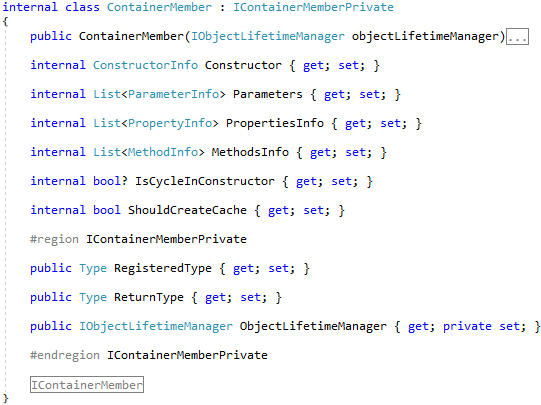
\includegraphics{ContainerMember.png}
  		\caption{Klasa ContainerMember}
  		\label{fig:ContainerMember}
	\end{center}
\end{figure}

Klasa ContainerMember przechowuje:
\begin{itemize}
	\item Informacje o konstruktorze, przy pomocy którego należy utworzyć obiekt danego typu.
	\item Informacje o parametrach tego konstruktora.
	\item Informacje o właściwościach danego typu (na potrzeby operacji BuildUp).
	\item Informacje o metodach danego typu (na potrzeby operacji BuildUp).
	\item Czy występuje cykl w konstruktorze.
	\item Czy należy zapamiętać informacje dla danego typu (domyślnie tak, dla typów zarejestrowanych jako Instance albo ObjectFactory - nie).
	\item Zarejestrowany typ (ta sama wartość, co klucz ze słownika).
	\item Zwracany typ.
	\item Informacje o menadżerze cyklu życia.
\end{itemize}

\subsubsection{Rozwiązanie 1 - PartialEmitFunction}
Cały algorytm jest zawarty w metodzie Resolve (Rys. \ref{fig:PartialEmitFunction_Resolve}). Sama ta metoda jest dość krótka, ale wywołuje ona kolejne metody (które już są dłuższe).\\
\\
Docelowy obiekt jest tworzony przy pomocy funkcji. Na początku następuje sprawdzenie, czy już wcześniej została utworzona taka funkcja (jeśli tak, będzie ona zapisana w klasie ContainerMember we właściwości ObjectLifetimeManager). Wywołanie funkcji kończy działanie algorytmu. Jeśli funkcja nie została wcześniej utworzona, to jest tworzona.\\
\\
Funkcja ta nie przyjmuje żadnych parametrów, a jej typem wynikowym jest obiekt. Ciało tej funkcji jest bardzo proste - po prostu ma ona wykonać metodę i zwrócić jej rezultat, którym jest nasz docelowy obiekt.\\ \\
\begin{figure}[H]
	\begin{center}
  		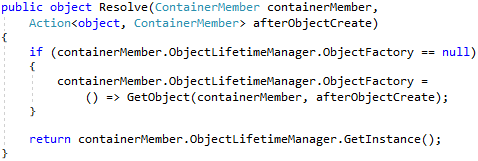
\includegraphics{PartialEmitFunction_Resolve.png}
  		\caption{Metoda Resolve klasy PartialEmitFunction}
  		\label{fig:PartialEmitFunction_Resolve}
	\end{center}
\end{figure}

Metoda GetObject (Rys. \ref{fig:PartialEmitFunction_GetObject}) jest trochę bardziej rozbudowana. Na początku są pobierane informacje o parametrach konstruktora danego typu. Następnie dla każdego z tych parametrów jest tworzony obiekt przy pomocy funkcji Resolve (opisanej wyżej). Została tutaj wykorzystana rekurencja. Gdy obiekty dla wszystkich parametrów konstruktora zostały utworzone, to ich lista jest przekazywana do metody CreateInstanceFunction, która zwraca instancję obiektu oczekiwanego typu. Na koniec jest wywoływana funkcja afterObjectCreate i docelowy obiekt zostaje zwrócony.\\ \\
\begin{figure}[H]
	\begin{center}
  		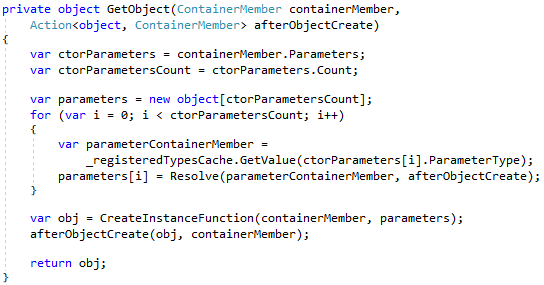
\includegraphics{PartialEmitFunction_GetObject.png}
  		\caption{Metoda GetObject klasy PartialEmitFunction}
  		\label{fig:PartialEmitFunction_GetObject}
	\end{center}
\end{figure}

Na początku metody CreateInstanceFunction (Rys. \ref{fig:PartialEmitFunction_CreateInstanceFunction}) występuje sprawdzenie, czy funkcja potrafiąca zwrócić obiekt docelowego typu, została utworzona.\\
\\
Jeśli tak, to przy pomocy tej funkcji jest tworzony obiekt, a następnie jest on zwracany. Ta funkcja jako argument przyjmuje listę obiektów w kolejności zgodnej z listą parametrów konstruktora.\\
\\
Jeśli nie, to przy pomocy metody CreateObjectFunction taka funkcja jest tworzona. W kolejnym kroku jest ona zapisywana w pamięci podręcznej (również w strukturze słownik, której kluczem jest typ, a wartością jest funkcja). Dalej dzieje się to samo, co w sytuacji, gdy ta funkcja jest już utworzona.\\ \\
\begin{figure}[H]
	\begin{center}
  		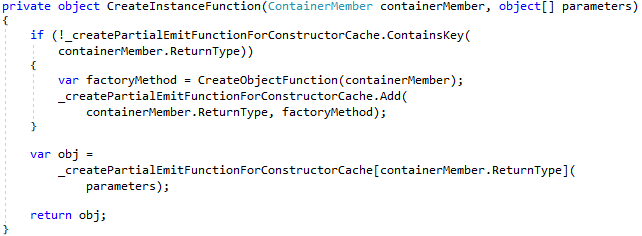
\includegraphics{PartialEmitFunction_CreateInstanceFunction.png}
  		\caption{Metoda CreateInstanceFunction klasy PartialEmitFunction}
  		\label{fig:PartialEmitFunction_CreateInstanceFunction}
	\end{center}
\end{figure}

CreateObjectFunction (Rys. \ref{fig:PartialEmitFunction_CreateObjectFunction}) jest najbardziej zaawansowaną metodą w tym algorytmie. To w niej wykorzystano metody z przestrzeni nazw Reflection.Emit.\\
\\
Na początku są pobierane informacje o konstruktorze. Następnie zostaje utworzony obiekt DynamicMethod i z niego jest pobierany ILGenerator. W nim będzie przechowywana listę kroków niezbędnych do utworzenia docelowego obiektu.\\
\\
Dla każdego z parametrów konstruktora są wykonane następujące operacje:
\begin{enumerate}
	\item Dodaj do listy kroków operację, która umieści na szczycie stosu pierwszy parametr (będzie nim lista obiektów zgodna z parametrami konstruktora).
	\item Dodaj do listy kroków operację, która umieści na szczycie stosu indeks parametru (który to jest parametr z kolei).
	\item Dodaj do listy kroków operację, która zdejmie ze szczytu stosu listę i indeks, a umieści na jego szczycie element znajdujący się pod danym indeksem na liście.
	\item Pobierz typ parametru.
	\item Dodaj do listy kroków operację, która zrzutuje obiekt ze szczytu stosu na odpowiedni typ.
\end{enumerate}
Po wykonaniu kroków z listy na stosie będą znajdowały się wszystkie obiekty, które są wymagane przez konstruktor do utworzenia danego typu. Teraz więc do listy kroków należy dodać jeszcze dwie operacje. Pierwsza z nich ma za zadanie stworzyć obiekt przy pomocy danego konstruktora i umieścić go na szczycie stosu. Druga ma na celu zwrócić obiekt ze szczytu stosu.\\
\\ \\
Wszystkie kroki niezbędne do stworzenia nowego elementu są zapisane w zmiennej typu DynamicMethod. Na końcu z tej zmiennej należy utworzyć, a następnie zwrócić delegata, który jako parametr będzie przyjmował tablicę obiektów (lista obiektów zgodna z parametrami konstruktora) i zwracał obiekt (docelowy obiekt).\\ \\
\begin{figure}[H]
	\begin{center}
  		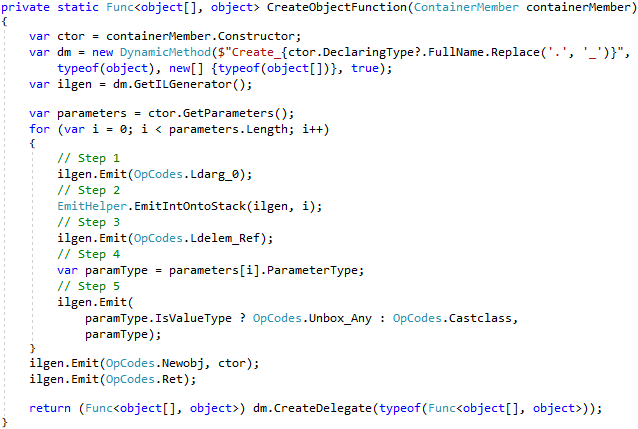
\includegraphics{PartialEmitFunction_CreateObjectFunction.png}
  		\caption{Metoda CreateObjectFunction klasy PartialEmitFunction}
  		\label{fig:PartialEmitFunction_CreateObjectFunction}
	\end{center}
\end{figure}

\subsubsection{Rozwiązanie 2 - FullEmitFunction}
Tutaj podobnie jak dla PartialEmitFunction cały algorytm zawarty jest w metodzie Resolve (Rys. \ref{fig:FullEmitFunction_Resolve}). Wygląda ona identycznie jak w rozwiązaniu 1 - docelowy obiekt jest tworzony przy pomocy funkcji, która woła w sobie metodę GetObject. Jeśli funkcji nie ma zapamiętanej w pamięci, to zostaje ona stworzona i zapisana. Na końcu jest ona wywoływana.\\ \\
\begin{figure}[H]
	\begin{center}
  		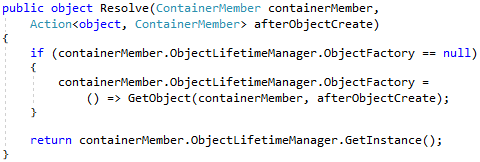
\includegraphics{FullEmitFunction_Resolve.png}
  		\caption{Metoda Resolve klasy FullEmitFunction}
  		\label{fig:FullEmitFunction_Resolve}
	\end{center}
\end{figure}

Metoda GetObject (Rys. \ref{fig:FullEmitFunction_GetObject}) wygląda trochę inaczej. Nie ma pobierania tutaj żadnych dodatkowych informacji, tylko od razu jest wywoływana metoda CreateInstanceFunction, która zwraca instancję obiektu oczekiwanego typu. Na koniec również jest wywoływana funkcja afterObjectCreate i zostaje zwrócony docelowy obiekt.\\ \\
\begin{figure}[H]
	\begin{center}
  		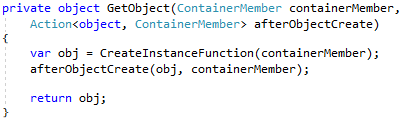
\includegraphics{FullEmitFunction_GetObject.png}
  		\caption{Metoda GetObject klasy FullEmitFunction}
  		\label{fig:FullEmitFunction_GetObject}
	\end{center}
\end{figure}

CreateInstanceFunction (Rys. \ref{fig:FullEmitFunction_CreateInstanceFunction}) ma jeden dodatkowy krok względem rozwiązania 1. Na początku również następuje sprawdzenie czy została wcześniej utworzona funkcja, która umie zwrócić obiekt docelowego typu. Jeśli nie, to przy pomocy metody CreateObjectFunction taka funkcja zostaje stworzona, a następnie jest zapisywana w pamięci podręcznej (również w strukturze słownika, którego kluczem jest typ, a wartością jest typ pomocniczy FullEmitFunctionResult, który ma tylko jedną właściwość - Result typu funkcja). Następnym krokiem jest walidacja zapisanych danych dla typów przy pomocy metody ValidateTypesCache. Na końcu funkcji obiekt jest tworzony, a następnie zwracany. Tutaj funkcja jako argument przyjmuje dwa słowniki. Pierwszy zawiera informacje o typie (kluczem jest typ, a wartością obiekt ContainerMember), a drugi informacje o indeksie typu (kluczem jest liczba oznaczając hasz danego typu, a wartością typ).\\

Najpierw zostanie opisana metoda ValidateTypesCache, ponieważ nie wywołuje ona w sobie żadnej innej metody.\\ \\
\begin{figure}[H]
	\begin{center}
  		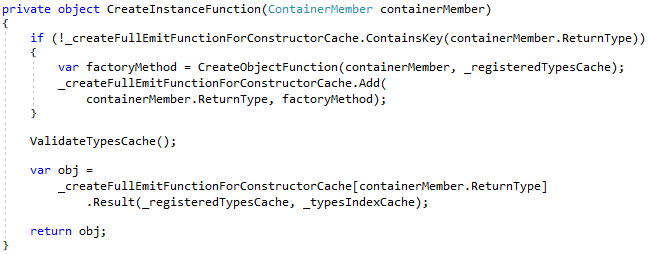
\includegraphics{FullEmitFunction_CreateInstanceFunction.png}
  		\caption{Metoda CreateInstanceFunction klasy FullEmitFunction}
  		\label{fig:FullEmitFunction_CreateInstanceFunction}
	\end{center}
\end{figure}

W pierwszym kroku metoda ValidateTypesCache sprawdza (Rys. \ref{fig:FullEmitFunction_ValidateTypesCache}), czy od ostatniego zapisywania danych o typach w pamięci podręcznej jakiś typ został zarejestrowany w kontenerze (lub czy jest to pierwsze zapisanie tych danych). Jeśli tak, to z zarejestrowanych typów zostaje utworzony słownik, w którym kluczem jest hasz typu, a wartością typ. Potem następuje aktualizacja liczby aktualnie zarejestrowanych typów.\\ \\
\begin{figure}[H]
	\begin{center}
  		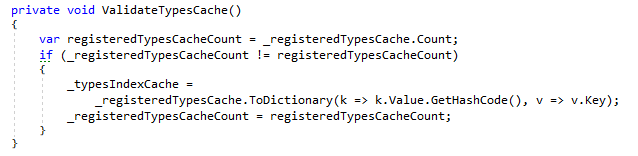
\includegraphics{FullEmitFunction_ValidateTypesCache.png}
  		\caption{Metoda ValidateTypesCache klasy FullEmitFunction}
  		\label{fig:FullEmitFunction_ValidateTypesCache}
	\end{center}
\end{figure}

Metoda CreateObjectFunction (Rys. \ref{fig:FullEmitFunction_CreateObjectFunction}) jest dużo bardziej rozbudowana niż w rozwiązaniu 1. W niej również są wykorzystane metody z przestrzeni nazw Reflection.Emit.\\
\\
Na początku jest tworzony obiekt typu DynamicMethod i z niego jest pobierany ILGenerator. W nim będzie przechowana lista kroków niezbędnych do utworzenia docelowego obiektu.\\
\\
Dla każdego z parametrów konstruktora jest wywoływana metoda CreateObjectFunctionPrivate, która uzupełnia listę kroków o tworzenie pośrednich obiektów. To w tym miejscu jest główna różnica między oboma rozwiązaniami - w pierwszym rozwiązaniu w liście kroków nie przejmowaliśmy się utworzeniem pośrednich obiektów, ponieważ przychodziły one jako parametr. W tym rozwiązaniu lista kroków będzie również zawierać niezbędne kroki do utworzenia wszystkich obiektów pośrednich (obiektów wymaganych przez konstruktor).\\
\\
Dalsze operacje są takie same jak w rozwiązaniu 1 - do listy kroków jest dodana operację, która stworzy obiekty przy pomocy danego konstruktora i umieści go na szczycie stosu, a następnie jest dodana operację, który zwróci nam obiekt ze szczytu stosu.\\
\\
Na końcu ze zmiennej typu DynamicMethod tworzony jest delegata, a następnie jest on zwracany. Delegat będzie przyjmował dwa parametry - oba typu Dictionary (słownik). Jeden z informacjami o typie, a drugi z informacjami o indeksie typu.\\ \\
\begin{figure}[H]
	\begin{center}
  		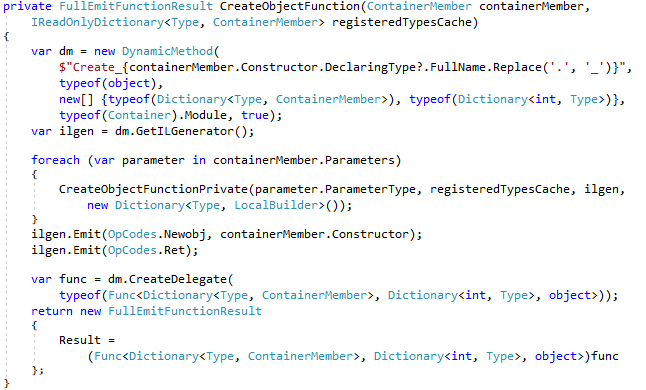
\includegraphics{FullEmitFunction_CreateObjectFunction.png}
  		\caption{Metoda CreateObjectFunction klasy FullEmitFunction}
  		\label{fig:FullEmitFunction_CreateObjectFunction}
	\end{center}
\end{figure}

W metodzie CreateObjectFunctionPrivate (Rys. \ref{fig:FullEmitFunction_CreateObjectFunctionPrivate}) są trzy przypadki. W pierwszych dwóch przypadkach pomijane są obiekty, które zostały zarejestrowane jako Instance albo FactoryObject (określa to parametr ShouldCreateCache z obiektu typu ContainerMember).\\
\begin{figure}[H]
	\begin{center}
  		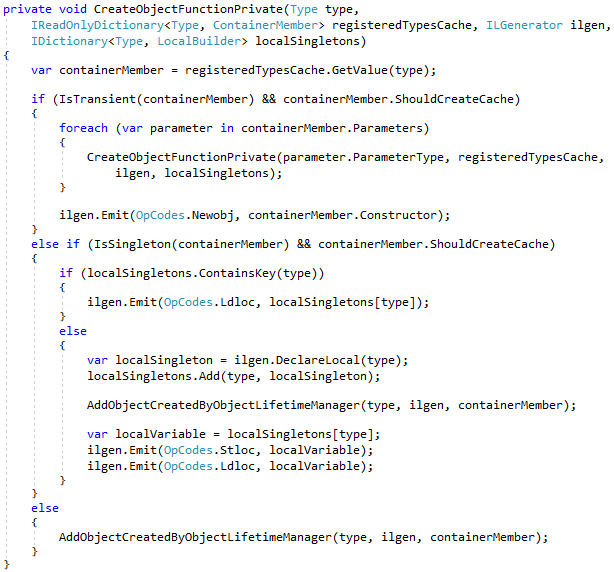
\includegraphics{FullEmitFunction_CreateObjectFunctionPrivate.png}
  		\caption{Metoda CreateObjectFunctionPrivate klasy FullEmitFunction}
  		\label{fig:FullEmitFunction_CreateObjectFunctionPrivate}
	\end{center}
\end{figure}

W pierwszym przypadku typ został zarejestrowany jako Transient -  Rys. \ref{fig:FullEmitFunction_IsTransient}. Dla każdego z parametrów konstruktora jest wywoływana rekurencyjnie ta metoda (CreateObjectFunctionPrivate), a na koniec do listy kroków jest dodawana operacja, która stworzy obiekty przy pomocy danego konstruktora i umieści go na szczycie stosu.\\ \\
\begin{figure}[H]
	\begin{center}
  		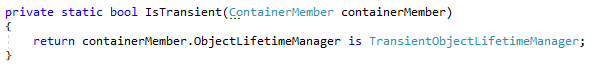
\includegraphics{FullEmitFunction_IsTransient.png}
  		\caption{Metoda IsTransient klasy FullEmitFunction}
  		\label{fig:FullEmitFunction_IsTransient}
	\end{center}
\end{figure}

W drugim przypadku typ musi być singletonem (został on zarejestrowany jako Singleton, PerThread lub PerHttpContext) -  Rys. \ref{fig:FullEmitFunction_IsSingleton}. Na początku następuje sprawdzenie czy już wcześniej algorytm natrafił na ten typ. Jeśli tak, to z pamięci podręcznej jest pobierana zmienna lokalna dla danego typu, a następnie do listy kroków jest dodawana operacja, która doda na szczyt stosu obiekt z tej zmiennej. Jeśli nie, to najpierw zostaje stworzona nową zmienna lokalna dla danego typu, a potem jest ona zapisywana w pamięci podręcznej (wykorzystany jest do tego słownik, gdzie kluczem jest typ, a wartością obiekt typu LocalBuilder). Następnie jest wywoływana metoda AddObjectCreatedByObjectLifetimeManager. Na końcu są dodawane dwie operacje. Pierwsza z nich zdejmie obiekt ze szczytu stosu i zapisze go w zmiennej lokalnej, a druga umieści na szczycie stosu obiekt z tej zmiennej lokalnej. Ma to na celu zapamiętanie danego obiektu i pozostawienie go na szczycie stosu. Dzięki takiemu zabiegowi, gdy drugi raz dany obiekt  będzie potrzebny (obiekt jest singletonem, więc za każdym razem będziemy chcieli mieć ten sam obiekt - w kontekście tworzenia danego typu, czyli jednej operacji Resolve), to z zapisanej zmiennej zostanie on dodany na szczyt stosu.\\ \\
\begin{figure}[H]
	\begin{center}
  		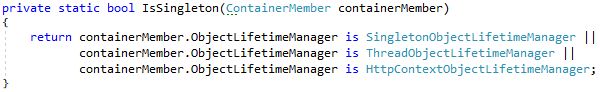
\includegraphics{FullEmitFunction_IsSingleton.png}
  		\caption{Metoda IsSingleton klasy FullEmitFunction}
  		\label{fig:FullEmitFunction_IsSingleton}
	\end{center}
\end{figure}

Metoda AddObjectCreatedByObjectLifetimeManager (Rys. \ref{fig:FullEmitFunction_AddObjectCreatedByObjectLifetimeManager}), za wyjątkiem pierwszej operacji jaką jest stworzenie zmiennej lokalnej typu Type, zawiera jedynie operacje, które dodają kolejne pozycje do listy kroków:
\begin{enumerate}
	\item Dodaj do listy kroków operację, która umieści na szczycie stosu drugi parametr (będzie nim słownik z indeksami typów).
	\item Dodaj do listy kroków operację, która umieści na szczycie stosu hasz danego typu.
	\item Dodaj do listy kroków operację, która pobierze ze szczytu stosu słownik i indeks, a umieści na jego szczycie element znajdujący się pod danym kluczem w słowniku.
	\item Dodaj do listy kroków operację, która zdejmie obiekt ze szczytu stosu i zapisze go w zmiennej lokalnej.
	\item Dodaj do listy kroków operację, która umieści na szczycie stosu pierwszy parametr (będzie nim słownik z informacjami o typach).
	\item Dodaj do listy kroków operację, która umieści na szczycie stosu obiekt ze zmiennej lokalnej.
	\item Dodaj do listy kroków operację, która zdejmie ze szczytu stosu słownik i typ, a umieści na jego szczycie element znajdujący się pod danym kluczem w słowniku.
	\item Dodaj do listy kroków operację, która zdejmie obiekt ze szczytu stosu (będzie to obiekt typu ContainerMember), wywoła na nim metodę, która zwróci menadżer czasu życia obiektu i na szczycie stosu umieści rezultat tej metody.
	\item Dodaj do listy kroków operację, która zdejmie obiekt ze szczytu stosu (będzie to obiekt typu IObjectLifeTimeManager), wywoła na nim metodę, która zwróci instancję obiektu i na szczycie stosu umieści rezultat tej metody.
	\item Dodaj do listy kroków operację, która zrzutuje obiekt ze szczytu stosu na odpowiedni typ.
\end{enumerate}
Po wykonaniu tych 10 operacji na szczycie stosu znajdzie się obiekt danego typu, który został utworzony przy pomocy odpowiedniego menadżera czasu życia.\\ \\
\begin{figure}[h]
	\begin{center}
  		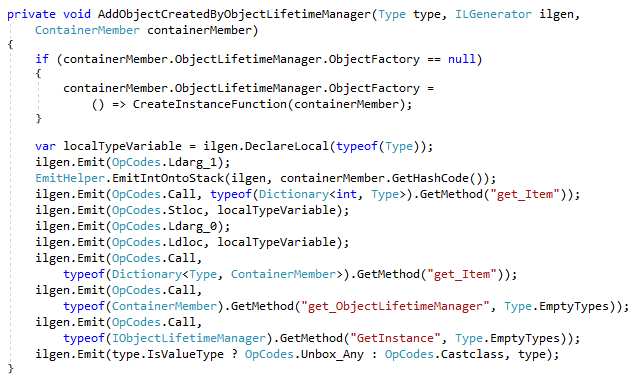
\includegraphics{FullEmitFunction_AddObjectCreatedByObjectLifetimeManager.png}
  		\caption{Metoda AddObjectCreatedByObjectLifetimeManager klasy FullEmitFunction}
  		\label{fig:FullEmitFunction_AddObjectCreatedByObjectLifetimeManager}
	\end{center}
\end{figure}

Trzeci przypadek zachodzi, gdy typ został zarejestrowany jako Instance, FactoryObject lub przy pomocy własnego menadżera czasu życia (własnej implementacji interfejsu IObjectLifetimeManager). W tej sytuacji zostaje wywołana tylko metoda AddObjectCreatedByObjectLifetimeManager.


\subsubsection{Przykład}
Mamy klasę A, która w konstruktorze przyjmuje obiekty klas B i C. Klasa B w konstruktorze przyjmuje obiekt klasy C, a klasa C ma konstruktor bezparametrowy. Tę sytuację przestawia Rys.  \ref{fig:Example_Classes}.\\ \\
\begin{figure}[H]
	\begin{center}
  		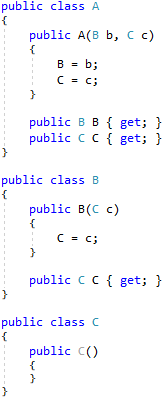
\includegraphics{Example_Classes.png}
  		\caption{Przykładowe klasy A, B i C}
  		\label{fig:Example_Classes}
	\end{center}
\end{figure}

Dla pierwszego rozwiązania (PartialEmitFunction), aby stworzyć obiekt klasy A, lista operacji IL prezentuje się następująco: \\
\\
// na stosie zostanie umieszona referencja do argumentu aktualnej funkcji, czyli do tablicy zawierającej B i C.\\
\texttt{ldarg\_0 [B, C]}\\
\\
// na stos zostanie dodana liczba 0.\\
\texttt{ldc\_i4\_0}\\
\\
// ze stosu zostanie ściągnięta liczba oraz tablica, a na jego szczycie zostanie umieszczony obiekt pod indeksem 0 z tablicy - w tym przypadku obiekt B.\\
\texttt{ldelem\_ref}\\
\\
// obiekt ze szczytu stosu jest rzutowany na typ B (wcześniej był typu object).\\
\texttt{castclass typeof(B)}\\
\\
// na stosie zostanie umieszona referencja do argumentu aktualnej funkcji, czyli do tablicy zawierającej B i C.\\
\texttt{ldarg\_0 [B, C]}\\
\\
//  na stos zostanie dodana liczba 1.\\
\texttt{ldc\_i4\_1}\\
\\
// ze stosu zostanie ściągnięta liczba oraz tablica, a na jego szczycie zostanie umieszczony obiekt pod indeksem 1 z tablicy - w tym przypadku obiekt C.\\
\texttt{ldelem\_ref}\\
\\
// obiekt ze szczytu stosu jest rzutowany na typ C.\\
\texttt{castclass typeof(C)}\\
\\
// ze stosu zostają zdjęcie wszystkie obiekty wymagane przez konstruktor klasy A (w tym przypadku obiekty B i C - muszą być one w odpowiedniej kolejności na stosie), a na jego szczycie jest umieszczany nowo utworzony obiekt A.\\
\texttt{newobj .ctor A}\\
\\
// obiekt ze szczytu stosu (obiekt A) zostaje zwrócony.\\
\texttt{ret} \\
\\
\\
Jak łatwo zauważyć, lista tych operacji zakłada, że mamy wcześniej stworzone obiekty wymagane w konstruktorze klasy A (w tym przypadku obiekty B i C). Te obiekty są tworzone na takiej samej zasadzie jak obiekt klasy A. Zatem w tym przypadku będziemy mieli 3 listy z operacjami IL - jedna dla obiektu C, jedna dla obiektu B i jedna dla obiektu A.\\
\\
Niezależnie od tego jak klasy A, B i C zostały zarejestrowane, zawsze uzyskamy dokładnie te same 3 listy operacji.\\
\\
\\
Dla drugiego rozwiązania (FullEmitFunction) jest to trochę bardziej rozbudowane.\\
\\
Jeśli wszystkie klasy zostały zarejestrowane jako Transient, to mamy krótką listę operacji:\\
\\ 
// na stosie zostanie umieszczony nowo utworzony obiekt C.\\
\texttt{newobj .ctor C}\\
\\
\newpage
// ze stosu zostanie zdjęty obiekt C i w jego miejsce pojawi się nowo utworzony obiekt B.\\
\texttt{newobj .ctor B}\\
\\ 
// na szczycie stosu zostanie umieszczony nowo utworzony obiekt C.\\
\texttt{newobj .ctor C}\\
\\
// ze szczytu stosu zostają zdjęcie obiekty B i C, a w ich miejsce pojawi się nowo utworzony obiekt A.\\
\texttt{newobj .ctor A}\\
\\
// obiekt ze szczytu stosu (obiekt A) zostaje zwrócony.\\
\texttt{ret}\\
\\
\\
Jeśli wszystkie klasy zostały zarejestrowane jako Singleton, PerThread lub PerHttpContext, to listę operacji wygląda następująco:\\
\\
// na stosie zostanie umieszona referencja do argumentu aktualnej funkcji, czyli do słownika zawierającego hash danego obiektu ContainerMember i typ obiektu.\\
\texttt{ldarg\_1 \{ \{1, typeof(A)\}, \{2, typeof(B)\}, \{3, typeof(C)\} \}}\\
\\
// na stos zostanie dodana liczba równa hashowi obiektu ContainerMember dla klasy B (w tym wypadku 2).\\
\texttt{ldc\_i4 2}\\
\\
//  ze stosu zostają pobrane dwa elementy (słownik oraz liczba), a następnie zostaje wywołana metoda "GetItem" na słowniku, której parametrem jest liczba. Wynik tej operacji (typ B) zostanie umieszczony na szczycie stosu.\\
\texttt{call "get\_Item"}\\
\\
// obiekt ze szczytu stosu zostaje zapisany w zmiennej variable\_Type\\
\texttt{stdloc variable\_Type}\\
\\
// na stosie zostanie umieszona referencja do argumentu aktualnej funkcji, czyli do słownika zawierającego typ obiektu i ContainerMember dla danego obiektu.\\
\texttt{ldarg\_0  \{ \{typeof(A), ContainerMember\}, \{typeof(B), ContainerMember\}, \{typeof(C), ContainerMember\}\}}\\
\\
// obiekt ze zmiennej variable\_Type zostaje umieszczony na szczycie stosu\\
\texttt{ldloc variable\_Type}\\
\\
\newpage
// ze stosu zostają pobrane dwa elementy (słownik oraz typ), a następnie zostaje wywołana metoda "GetItem" na słowniku, której parametrem jest typ. Wynik tej operacji (obiekt ContainerMember dla typu B) zostanie umieszczony na szczycie stosu.\\
\texttt{call "get\_Item" }\\
\\
// ze stosu zostaje pobrany element i jest na nim wywołana metoda GetObjectLifetimeManager. Wynik tej operacji (odpowiedni obiekt ObjectLifetimeManager) zostanie umieszczony na szczycie stosu.\\
\texttt{call "get\_ObjectLifetimeManager"}\\
\\
// ze stosu zostaje pobrany element i jest na nim wywołana metoda GetInstance. Wynik tej operacji (obiekt typu B) zostanie umieszczony na szczycie stosu.\\
\texttt{call "GetInstance"}\\
\\
// obiekt ze szczytu stosu jest rzutowany na typ B.\\
\texttt{castclass}\\
\\
// obiekt ze szczytu stosu zostaje zapisany w zmiennej variable\_B\\
\texttt{stloc variable\_B}\\
\\
// obiekt ze zmiennej variable\_B zostaje umieszczony na szczycie stosu\\
\texttt{ldloc variable\_B}\\
\\
\texttt{ldarg\_1 \{ \{1, typeof(A)\}, \{2, typeof(B)\}, \{3, typeof(C)\} \}}\\
\\
// na stos zostanie dodana liczba równa hashowi obiektu ContainerMember dla klasy C (w tym wypadku 3).\\
\texttt{ldc\_i4 3}\\
\\
// ze stosu zostają pobrane dwa elementy (słownik oraz liczba), a następnie zostaje wywołana metoda "GetItem" na słowniku, której parametrem jest liczba. Wynik tej operacji (typ C) zostanie umieszczony na szczycie stosu.\\
\texttt{call "get\_Item"}\\
\\
// obiekt ze szczytu stosu zostaje zapisany w zmiennej variable\_Type\\
\texttt{stdloc variable\_Type}\\
\\
\texttt{ldarg\_o  \{ \{typeof(A), ContainerMember\}, \{typeof(B), ContainerMember\}, \{typeof(C), ContainerMember\}\}}\\
\\
// obiekt ze zmiennej variable\_Type zostaje umieszczony na szczycie stosu\\
\texttt{ldloc variable\_Type}\\
\\
\newpage
// ze stosu zostają pobrane dwa elementy (słownik oraz typ), a następnie zostaje wywołana metoda "GetItem" na słowniku, której parametrem jest typ. Wynik tej operacji (obiekt ContainerMember dla typu C) zostanie umieszczony na szczycie stosu.\\
\texttt{call "get\_Item"}\\
\\
// ze stosu zostaje pobrany element i jest na nim wywołana metoda GetObjectLifetimeManager. Wynik tej operacji (odpowiedni obiekt ObjectLifetimeManager) zostanie umieszczony na szczycie stosu.\\
\texttt{call "get\_ObjectLifetimeManager"}\\
\\
// ze stosu zostaje pobrany element i jest na nim wywołana metoda GetInstance. Wynik tej operacji (obiekt typu C) zostanie umieszczony na szczycie stosu.\\
\texttt{call "GetInstance"}\\
\\
// obiekt ze szczytu stosu jest rzutowany na typ C.\\
\texttt{castclass}\\
\\
// obiekt ze szczytu stosu zostaje zapisany w zmiennej variable\_C\\
\texttt{stloc variable\_C}\\
\\
// obiekt ze zmiennej variable\_C zostaje umieszczony na szczycie stosu\\
\texttt{ldloc variable\_C}\\
\\
// ze szczytu stosu zostają zdjęcie obiekty B i C, a w ich miejsce pojawi się nowo utworzony obiekt A\\
\texttt{newobj .ctor A}\\
\\
// obiekt ze szczytu stosu (obiekt A) zostaje zwrócony\\
\texttt{ret}\\
\\
\\
Jeśli typ został zarejestrowany jako Instance, FactoryObject albo z własną implementacją interfejsu IObjectLifetimeManager, to lista kroków wygląda podobnie jak dla Singleton, z tą różnicą, że nie ma kroków z zapisywaniem obiektu do zmiennej lokalnej (w tym przypadku brak kroków 11, 12, 23 i 24).



\clearpage
\section{Testy wydajnościowe}
Do przeprowadzania testów wydajnościowych przygotowano osobną aplikację, w której zostały utworzone 4 przypadki testowe:
\begin{itemize}
	\item Przypadek testowy A,
	\item Przypadek testowy B,
	\item Przypadek testowy C,
	\item Przypadek testowy D.
\end{itemize}
Dla każdego z przypadków sprawdzany jest czas wykonania operacji "Resolve" dla różnych rodzajów rejestracji. Testy zostały wykonane dla następujących wariantów rejestracji:
\begin{itemize}
	\item Register as Singleton,
	\item Register as Transient,
	\item Register as TransientSingleton,
	\item Register as PerThread (dla niektórych przemysłowych rozwiązań - PerScope),
	\item Register as FactoryMethod.
\end{itemize}
Każdy z testów dla każdego rozwiązania był uruchamiany w osobnym procesie. Wynika dla operacji "Register" zostały pominięte, ponieważ są one prawie zawsze mniejsze niż 1 ms. Przy operacji "Resolve" każdy test był uruchamiany 100 razy, a w wynikach zostały przedstawione następujące czasy w milisekundach: minimalny, maksymalny i średni. Dla pierwszych trzech przypadków testy były wykonywane dla: 1, 10, 100 i 1000 powtórzeń, a dla ostatniego przypadku dla: 1 i 10 powtórzeń.

\subsubsection{Register as Singleton}
Każdy typ jest zarejestrowany jako "Singleton", czyli obiekt jest tworzony raz, a następnie cały czas zwracany.

\subsubsection{Register as Transient}
Każdy typ jest zarejestrowany jako "Transient", czyli za każdym razem jest tworzony nowy obiekt.

\subsubsection{Register as TransientSingleton}
Każdy typ jest zarejestrowany jako "Transient" za wyjątkiem typów, które maja konstruktor bezparametrowy - są one zarejestrowane jako "Singleton".

\subsubsection{Register as PerThread}
Każdy typ jest zarejestrowany jako "PerThread", czyli obiekt jest tworzony raz dla każdego wątku, a następnie w obrębie tego wątku cały czas zwracany.

\subsubsection{Register as FactoryMethod}
Każdy typ jest zarejestrowany jako "FactoryMethod", czyli jako funkcja, która zwraca nam obiekt danego typu. Ciało tej funkcji wygląda tak, że oczekiwany typ jest tworzony z użyciem konstruktora (za pomocą "new"), a wszystkie parametry wymagane przez ten konstruktor są tworzone przy pomocy operacji Resolve.


\subsection{Przypadek testowy A}
\subsubsection{Opis}
W tym teście mamy zdefiniowanych 11 typów. Każdy z nich przyjmuje w konstruktorze o jeden parametr mniej niż typ poprzedni (czyli przyjmują one kolejno od 10 do 0 parametrów w konstruktorze). Typem głównym, a zarazem typem o największej liczbie parametrów, jest typ "TestA". Przyjmuje on w konstruktorze 10 parametrów następujących typów: "TestA0", "TestA1", "TestA2", "TestA3", "TestA4", "TestA5", "TestA6", "TestA7", "TestA8", "TestA9". Każdy z tych 10 typów w konstruktorze przyjmuje tyle parametrów, ile wynosi liczba w jego nazwie (czyli obiekt typu "TestA0" ma konstruktor bezparametrowy, obiekt typy "TestA1" ma konstruktor z jednym parametrem; i tak dalej aż do typu "TestA9", który ma konstruktor z dziewięcioma parametrami). Wszystkie typy jako parametry w konstruktorze przyjmują obiekty typów z niższymi liczbami w nazwie (czyli obiekt typu "TestA1" w konstruktorze przyjmuje obiekt typu "TestA0", obiekt typu "TestA2" przyjmuje w konstruktorze obiekty typów "TestA0" i "TestA1"; i tak dalej aż do typu "TestA9", który w konstruktorze przyjmuje obiekty z typami od "TestA0" do "TestA8"). Graf zależności poszczególnych typów został przedstawiony na Rys. \ref{fig:testA}.\\
\begin{figure}[H]
	\begin{center}
  		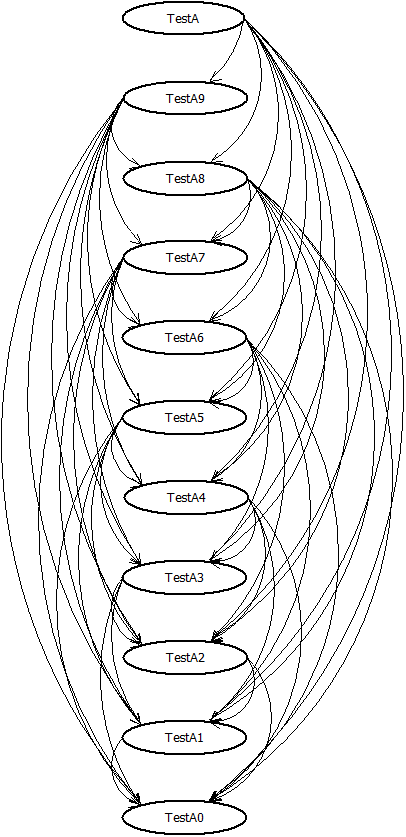
\includegraphics[height=11.5cm]{TestA.png}
  		\caption{Graf zależności dla testu A.}
  		\label{fig:testA}
	\end{center}
\end{figure}

Łatwo z niego wywnioskować, że tworząc obiekty poszczególnych typów liczba tworzonych obiektów rośnie wykładniczo:
\begin{itemize}
	\item TestA0 - 1 obiekt,
	\item TestA1 - 2 obiekty (obiekt typu TestA1 i obiekt typu TestA0),
	\item TestA2 - 4 obiekty (obiekt typu TestA2, obiekt typu TestA1 - 2 obiekty, obiekt typu TestA0 - 1 obiekt),
	\item TestA3 - 8 obiektów (obiekt typu TestA3, obiekt typu TestA2 - 4 obiekty, obiekt typu TestA1 - 2 obiekty, obiekt typu TestA0 - 1 obiekt),
	\item TestA4 - 16 obiektów,
	\item TestA5 - 32 obiektów,
	\item TestA6 - 64 obiektów,
	\item TestA7 - 128 obiektów,
	\item TestA8 - 256 obiektów,
	\item TestA9 - 512 obiektów,
	\item TestA - 1 024 obiektów.
\end{itemize}
Zatem tworząc nasz główny obiekt typu TestA, tworzymy: 1 obiekt typu TestA, 1 obiekt typu TestA9, 2 obiekty typu TestA8, 4 obiekty typu TestA7, 8 obiektów typu TestA6, 16 obiektów typu TestA5, 32 obiektów typu TestA4, 64 obiektów typu TestA3, 128 obiektów typu TestA2, 256 obiektów typu TestA1 i 512 obiektów typu TestA0 - co w sumie daje 1024 obiekty.

\subsubsection{Wyniki Resolve dla Singleton}
\begin{table}[H]
\captionsetup{belowskip=0pt,aboveskip=0pt}
\begin{center}
\begin{small}
	\begin{tabular}{ | l | r r r | }
    		\hline
Liczba & & 1 & \\ \hline
 & min & max & avg \\ \hline
Autofac & 0 & 0 & 0 \\ \hline
Windsor & 0 & 0 & 0 \\ \hline
NiquIoCPartial & 1 & 1 & 1 \\ \hline
DryIoc & 2 & 2 & 2 \\ \hline
Grace & 2 & 2 & 2 \\ \hline
LightInject & 2 & 2 & 2 \\ \hline
NiquIoCFull & 2 & 2 & 2 \\ \hline
SimpleInjector & 2 & 2 & 2 \\ \hline
Ninject & 3 & 3 & 3 \\ \hline
Unity & 7 & 8 & 7 \\ \hline
StructureMap & 9 & 10 & 9 \\ \hline
  	\end{tabular}
\end{small}
\end{center}
\caption{Wyniki testów dla 1 powtórzenia dla operacji Singleton dla Przypadku testowego A}
\label{TestCaseA_Singleton1}
\end{table}
Czasy dla wszystkich rozwiązań są nieduże. Jest to spowodowane tym, że gdy wszystkie klasy są zarejestrowane jako Singleton, to jest tworzonych niewiele nowych obiektów.\\
\\
Należy jednak wspomnieć, że najsłabiej tutaj  poradziły sobie Unity i StructureMap, których czasy są zauważalnie większe niż pozostałych rozwiązań.
\\ \\
\begin{table}[H]
\captionsetup{belowskip=0pt,aboveskip=0pt}
\begin{center}
\begin{small}
	\begin{tabular}{ | l | r r r | }
    		\hline
Liczba & & 1000 & \\ \hline
 & min & max & avg \\ \hline
Autofac & 0 & 0 & 0 \\ \hline
Windsor & 0 & 0 & 0 \\ \hline
NiquIoCPartial & 1 & 1 & 1 \\ \hline
DryIoc & 2 & 2 & 2 \\ \hline
LightInject & 2 & 2 & 2 \\ \hline
NiquIoCFull & 2 & 2 & 2 \\ \hline
SimpleInjector & 2 & 2 & 2 \\ \hline
Grace & 2 & 3 & 2 \\ \hline
Ninject & 6 & 7 & 6 \\ \hline
Unity & 8 & 8 & 8 \\ \hline
StructureMap & 10 & 11 & 10 \\ \hline
  	\end{tabular}
\end{small}
\end{center}
\caption{Wyniki testów dla 1000 powtórzeń dla operacji Singleton dla Przypadku testowego A}
\label{TestCaseA_Singleton1000}
\end{table}
Gdy klasa jest zarejestrowana jako Singleton, to wraz ze wzrostem liczby tworzonych obiektów, nie powinien wzrastać czas ich tworzenia. We wszystkich rozwiązaniach, za wyjątkiem Ninject, czasy dla 1000 operacji, są zbliżone do czasów dla 1 operacji. Ninject natomiast ma czasy około dwa razy większe.

\subsubsection{Wyniki Resolve dla Transient}
\begin{table}[H]
\captionsetup{belowskip=0pt,aboveskip=0pt}
\begin{center}
\begin{small}
	\begin{tabular}{ | l | r r r | }
    		\hline
Liczba & & 1 & \\ \hline
 & min & max & avg \\ \hline
Autofac & 0 & 0 & 0 \\ \hline
NiquIoCPartial & 1 & 1 & 1 \\ \hline
Windsor & 1 & 2 & 1 \\ \hline
NiquIoCFull & 8 & 9 & 8 \\ \hline
Unity & 8 & 9 & 8 \\ \hline
LightInject & 10 & 10 & 10 \\ \hline
StructureMap & 10 & 10 & 10 \\ \hline
Ninject & 10 & 12 & 11 \\ \hline
SimpleInjector & 13 & 14 & 13 \\ \hline
DryIoc & 14 & 14 & 14 \\ \hline
Grace & 15 & 16 & 15 \\ \hline
  	\end{tabular}
\end{small}
\end{center}
\caption{Wyniki testów dla 1 powtórzenia dla operacji Transient dla Przypadku testowego A}
\label{TestCaseA_Transient1}
\end{table}
W tym wypadku najlepiej poradziły sobie Autofac, NiquIoCPartial i Windsor, które uzyskały zbliżone rezultaty. Pozostałe rozwiązania uzyskały dużo słabsze, o kilka razy większe czasy.
\\ \\
\begin{table}[H]
\captionsetup{belowskip=0pt,aboveskip=0pt}
\begin{center}
\begin{small}
	\begin{tabular}{ | l | r r r | }
    		\hline
Liczba & & 10 & \\ \hline
 & min & max & avg \\ \hline
NiquIoCPartial & 3 & 3 & 3 \\ \hline
Autofac & 6 & 7 & 6 \\ \hline
NiquIoCFull & 8 & 9 & 8 \\ \hline
LightInject & 10 & 10 & 10 \\ \hline
SimpleInjector & 13 & 14 & 14 \\ \hline
StructureMap & 13 & 14 & 14 \\ \hline
DryIoc & 14 & 15 & 15 \\ \hline
Grace & 15 & 16 & 16 \\ \hline
Unity & 16 & 17 & 16 \\ \hline
Windsor & 16 & 21 & 16 \\ \hline
Ninject & 88 & 95 & 90 \\ \hline
  	\end{tabular}
\end{small}
\end{center}
\caption{Wyniki testów dla 10 powtórzeń dla operacji Transient dla Przypadku testowego A}
\label{TestCaseA_Transient10}
\end{table} 
Najmniejszy czas uzyskał NiquIoCPartial, ale jest on niestety kilkukrotnie większy niż dla 1 powtórzenia. Co więcej wszystkie najpopularniejsze rozwiązania zanotowały spory wzrost czasów. Z drugiej strony wszystkie najszybsze rozwiązania oraz NiquIoCFull zanotowały podobne czasy co dla 1 powtórzenia.
\\ \\
\begin{table}[H]
\captionsetup{belowskip=0pt,aboveskip=0pt}
\begin{center}
\begin{small}
	\begin{tabular}{ | l | r r r | }
    		\hline
Liczba & & 100 & \\ \hline
 & min & max & avg \\ \hline
NiquIoCFull & 9 & 10 & 9 \\ \hline
LightInject & 11 & 12 & 11 \\ \hline
SimpleInjector & 15 & 15 & 15 \\ \hline
DryIoc & 16 & 16 & 16 \\ \hline
Grace & 18 & 19 & 18 \\ \hline
NiquIoCPartial & 19 & 22 & 19 \\ \hline
StructureMap & 53 & 55 & 54 \\ \hline
Autofac & 58 & 63 & 59 \\ \hline
Unity & 88 & 91 & 88 \\ \hline
Windsor & 152 & 192 & 155 \\ \hline
Ninject & 864 & 1035 & 882 \\ \hline
  	\end{tabular}
\end{small}
\end{center}
\caption{Wyniki testów dla 100 powtórzeń dla operacji Transient dla Przypadku testowego A}
\label{TestCaseA_Transient100}
\end{table}
Wraz ze wzrostem liczby powtórzeń coraz słabiej radzi sobie NiquIoCPartial oraz najpopularniejsze rozwiązania. Wszystkie one notują spory wzrost czasów. Dla NiquIoCFull i najszybszych rozwiązań ten wzrost jest nieznaczny.
\\ \\
\begin{table}[H]
\captionsetup{belowskip=0pt,aboveskip=0pt}
\begin{center}
\begin{small}
	\begin{tabular}{ | l | r r r | }
    		\hline
Liczba & & 1000 & \\ \hline
 & min & max & avg \\ \hline
NiquIoCFull & 18 & 19 & 18 \\ \hline
LightInject & 19 & 20 & 19 \\ \hline
SimpleInjector & 28 & 30 & 29 \\ \hline
DryIoc & 29 & 30 & 29 \\ \hline
Grace & 37 & 38 & 37 \\ \hline
NiquIoCPartial & 171 & 198 & 173 \\ \hline
StructureMap & 414 & 457 & 417 \\ \hline
Autofac & 584 & 609 & 587 \\ \hline
Unity & 803 & 961 & 813 \\ \hline
Windsor & 1511 & 1799 & 1529 \\ \hline
Ninject & 8745 & 9610 & 8934 \\ \hline
  	\end{tabular}
\end{small}
\end{center}
\caption{Wyniki testów dla 1000 powtórzeń dla operacji Transient dla Przypadku testowego A}
\label{TestCaseA_Transient1000}
\end{table}
Test dla 1000 powtórzeń potwierdził, że czasy dla NiquIoCPartial oraz najpopularniejszych rozwiązań rosną liniowo wraz ze wzrostem liczby powtórzeń. Czasy dla NiquIoCFull oraz najszybszych rozwiązań również wzrosły, ale zaledwie dwukrotnie w stosunku do dziesięciokrotnego wzrostu liczby powtórzeń.

\subsubsection{Wyniki Resolve dla TransientSingleton}
\begin{table}[H]
\captionsetup{belowskip=0pt,aboveskip=0pt}
\begin{center}
\begin{small}
	\begin{tabular}{ | l | r r r | }
    		\hline
Liczba & & 1 & \\ \hline
 & min & max & avg \\ \hline
Autofac & 0 & 0 & 0 \\ \hline
NiquIoCPartial & 1 & 1 & 1 \\ \hline
Windsor & 1 & 2 & 1 \\ \hline
NiquIoCFull & 5 & 6 & 5 \\ \hline
Unity & 8 & 9 & 8 \\ \hline
SimpleInjector & 9 & 9 & 9 \\ \hline
Grace & 9 & 10 & 10 \\ \hline
Ninject & 9 & 10 & 10 \\ \hline
StructureMap & 9 & 10 & 10 \\ \hline
LightInject & 14 & 15 & 14 \\ \hline
DryIoc & 18 & 19 & 18 \\ \hline
  	\end{tabular}
\end{small}
\end{center}
\caption{Wyniki testów dla 1 powtórzenia dla operacji TransientSingleton dla Przypadku testowego A}
\label{TestCaseA_TransientSingleton1}
\end{table}
Dla 1 powtórzenia najmniejsze czasy uzyskały NiquIoCPartial oraz najpopularniejsze rozwiązania.
\\ \\
\begin{table}[H]
\captionsetup{belowskip=0pt,aboveskip=0pt}
\begin{center}
\begin{small}
	\begin{tabular}{ | l | r r r | }
    		\hline
Liczba & & 10 & \\ \hline
 & min & max & avg \\ \hline
NiquIoCPartial & 2 & 3 & 2 \\ \hline
NiquIoCFull & 5 & 6 & 5 \\ \hline
Autofac & 6 & 7 & 6 \\ \hline
SimpleInjector & 9 & 10 & 9 \\ \hline
Grace & 10 & 10 & 10 \\ \hline
StructureMap & 12 & 12 & 12 \\ \hline
Windsor & 12 & 14 & 12 \\ \hline
LightInject & 14 & 14 & 14 \\ \hline
Unity & 14 & 15 & 14 \\ \hline
DryIoc & 19 & 19 & 19 \\ \hline
Ninject & 65 & 82 & 67 \\ \hline
  	\end{tabular}
\end{small}
\end{center}
\caption{Wyniki testów dla 10 powtórzeń dla operacji TransientSingleton dla Przypadku testowego A}
\label{TestCaseA_TransientSingleton10}
\end{table}
Gdy mamy 10 powtórzeń czasy wszystkich rozwiązań wydają się być do siebie zbliżone. Wyjątkiem są tylko dwa rozwiązania: NiquIoCPartial razy sobie trochę lepiej niż pozostałe, a Ninject trochę słabiej.
\\ \\
\begin{table}[H]
\captionsetup{belowskip=0pt,aboveskip=0pt}
\begin{center}
\begin{small}
	\begin{tabular}{ | l | r r r | }
    		\hline
Liczba & & 100 & \\ \hline
 & min & max & avg \\ \hline
NiquIoCFull & 6 & 6 & 6 \\ \hline
SimpleInjector & 10 & 11 & 10 \\ \hline
Grace & 10 & 11 & 11 \\ \hline
NiquIoCPartial & 14 & 15 & 14 \\ \hline
LightInject & 14 & 15 & 15 \\ \hline
DryIoc & 20 & 21 & 20 \\ \hline
StructureMap & 35 & 40 & 36 \\ \hline
Autofac & 53 & 62 & 54 \\ \hline
Unity & 73 & 82 & 74 \\ \hline
Windsor & 117 & 140 & 119 \\ \hline
Ninject & 626 & 743 & 641 \\ \hline
  	\end{tabular}
\end{small}
\end{center}
\caption{Wyniki testów dla 100 powtórzeń dla operacji TransientSingleton dla Przypadku testowego A}
\label{TestCaseA_TransientSingleton100}
\end{table}
W teście również gdy liczba powtórzeń wzrosła do 100, to najlepsze czasy zaczęły uzyskiwać NiquIoCFull i najszybsze rozwiązania. NiquIoCPartial oraz najpopularniejsze rozwiązania zanotował kilkukrotny wzrost czasów.
\\ \\
\begin{table}[H]
\captionsetup{belowskip=0pt,aboveskip=0pt}
\begin{center}
\begin{small}
	\begin{tabular}{ | l | r r r | }
    		\hline
Liczba & & 1000 & \\ \hline
 & min & max & avg \\ \hline
NiquIoCFull & 10 & 12 & 11 \\ \hline
SimpleInjector & 17 & 19 & 17 \\ \hline
Grace & 18 & 19 & 18 \\ \hline
LightInject & 20 & 21 & 20 \\ \hline
DryIoc & 31 & 32 & 32 \\ \hline
NiquIoCPartial & 120 & 123 & 121 \\ \hline
StructureMap & 252 & 306 & 256 \\ \hline
Autofac & 531 & 561 & 535 \\ \hline
Unity & 659 & 753 & 663 \\ \hline
Windsor & 1161 & 1302 & 1177 \\ \hline
Ninject & 6297 & 7218 & 6463 \\ \hline
  	\end{tabular}
\end{small}
\end{center}
\caption{Wyniki testów dla 1000 powtórzeń dla operacji TransientSingleton dla Przypadku testowego A}
\label{TestCaseA_TransientSingleton1000}
\end{table}
Przy 1000 powtórzeń NiquIoCFull oraz wszystkie najszybsze rozwiązania uzyskały czasy o rząd wielkości mniejsze niż NiquIoCParial i najpopularniejsze rozwiązania.

\subsubsection{Wyniki Resolve dla PerThread}
\begin{table}[H]
\captionsetup{belowskip=0pt,aboveskip=0pt}
\begin{center}
\begin{small}
	\begin{tabular}{ | l | r r r | }
    		\hline
Liczba & & 1 & \\ \hline
 & min & max & avg \\ \hline
Autofac & 0 & 0 & 0 \\ \hline
Windsor & 0 & 0 & 0 \\ \hline
NiquIoCPartial & 1 & 1 & 1 \\ \hline
NiquIoCFull & 2 & 2 & 2 \\ \hline
Ninject & 3 & 3 & 3 \\ \hline
Grace & 4 & 4 & 4 \\ \hline
Unity & 7 & 8 & 7 \\ \hline
SimpleInjector & 7 & 8 & 8 \\ \hline
StructureMap & 9 & 10 & 9 \\ \hline
LightInject & 50 & 53 & 50 \\ \hline
DryIoc & 71 & 73 & 71 \\ \hline
  	\end{tabular}
\end{small}
\end{center}
\caption{Wyniki testów dla 1 powtórzenia dla operacji PerThread dla Przypadku testowego A}
\label{TestCaseA_PerThread1}
\end{table}
Z racji tego, że wszystkie obiekty są tworzone w jednym wątku czasy powinny być zbliżone do wyników operacji resolve dla Singleton. Za wyjątkiem dwóch rozwiązań - LightInject i DryIoc, wszystkie pozostałe uzyskały zbliżone czasy. Te dwa rozwiązania najwyraźniej nie radzą sobie dla tego typu rejestracji.
\\ \\
\begin{table}[H]
\captionsetup{belowskip=0pt,aboveskip=0pt}
\begin{center}
\begin{small}
	\begin{tabular}{ | l | r r r | }
    		\hline
Liczba & & 1000 & \\ \hline
 & min & max & avg \\ \hline
Autofac & 0 & 0 & 0 \\ \hline
Windsor & 0 & 0 & 0 \\ \hline
NiquIoCPartial & 1 & 1 & 1 \\ \hline
NiquIoCFull & 2 & 2 & 2 \\ \hline
Grace & 4 & 4 & 4 \\ \hline
Ninject & 6 & 7 & 6 \\ \hline
SimpleInjector & 8 & 8 & 8 \\ \hline
Unity & 8 & 9 & 8 \\ \hline
StructureMap & 10 & 10 & 10 \\ \hline
LightInject & 50 & 52 & 51 \\ \hline
DryIoc & 72 & 74 & 72 \\ \hline
  	\end{tabular}
\end{small}
\end{center}
\caption{Wyniki testów dla 1000 powtórzeń dla operacji PerThread dla Przypadku testowego A}
\label{TestCaseA_PerThread1000}
\end{table}
Podobnie jak w przypadku resolve dla Singleton, tutaj również wzrost liczby powtórzeń nie miał wpływu na wzrost czasu.

\subsubsection{Wyniki Resolve dla FactoryMethod}
\begin{table}[H]
\captionsetup{belowskip=0pt,aboveskip=0pt}
\begin{center}
\begin{small}
	\begin{tabular}{ | l | r r r | }
    		\hline
Liczba & & 1 & \\ \hline
 & min & max & avg \\ \hline
Autofac & 0 & 0 & 0 \\ \hline
DryIoc & 0 & 0 & 0 \\ \hline
LightInject & 0 & 0 & 0 \\ \hline
NiquIoCPartial & 0 & 0 & 0 \\ \hline
NiquIoCFull & 0 & 0 & 0 \\ \hline
SimpleInjector & 1 & 1 & 1 \\ \hline
Unity & 1 & 1 & 1 \\ \hline
Windsor & 1 & 1 & 1 \\ \hline
Grace & 2 & 2 & 2 \\ \hline
StructureMap & 7 & 7 & 7 \\ \hline
Ninject & 8 & 10 & 9 \\ \hline
  	\end{tabular}
\end{small}
\end{center}
\caption{Wyniki testów dla 1 powtórzenia dla operacji FactoryMethod dla Przypadku testowego A}
\label{TestCaseA_FactoryMethod1}
\end{table}
Dla tego testu dla 1 powtórzenia wszystkie rozwiązania za wyjątkiem StructureMap i Ninject uzyskały zbliżone rezultaty. Te dwa rozwiązania poradziły sobie słabiej niż reszta.
\begin{table}[H]
\captionsetup{belowskip=0pt,aboveskip=0pt}
\begin{center}
\begin{small}
	\begin{tabular}{ | l | r r r | }
    		\hline
Liczba & & 10 & \\ \hline
 & min & max & avg \\ \hline
DryIoc & 0 & 0 & 0 \\ \hline
LightInject & 1 & 1 & 1 \\ \hline
NiquIoCPartial & 1 & 1 & 1 \\ \hline
NiquIoCFull & 1 & 1 & 1 \\ \hline
SimpleInjector & 2 & 2 & 2 \\ \hline
Grace & 3 & 5 & 3 \\ \hline
Autofac & 5 & 8 & 6 \\ \hline
Windsor & 10 & 11 & 10 \\ \hline
StructureMap & 11 & 11 & 11 \\ \hline
Unity & 14 & 15 & 14 \\ \hline
Ninject & 53 & 60 & 55 \\ \hline
  	\end{tabular}
\end{small}
\end{center}
\caption{Wyniki testów dla 10 powtórzeń dla operacji FactoryMethod dla Przypadku testowego A}
\label{TestCaseA_FactoryMethod10}
\end{table}
Wraz ze wzrostem liczby powtórzeń tym razem również wszystkie najpopularniejsze rozwiązania zanotowały liniowy wzrost czasów. Oba rozwiązania przedstawione w tej pracy oraz wszystkie najszybsze rozwiązania uzyskały zbliżone wyniki.
\\ \\
\begin{table}[H]
\captionsetup{belowskip=0pt,aboveskip=0pt}
\begin{center}
\begin{small}
	\begin{tabular}{ | l | r r r | }
    		\hline
Liczba & & 100 & \\ \hline
 & min & max & avg \\ \hline
DryIoc & 6 & 6 & 6 \\ \hline
LightInject & 6 & 8 & 7 \\ \hline
NiquIoCFull & 11 & 12 & 12 \\ \hline
SimpleInjector & 11 & 12 & 12 \\ \hline
NiquIoCPartial & 12 & 12 & 12 \\ \hline
Grace & 12 & 13 & 12 \\ \hline
Autofac & 49 & 57 & 50 \\ \hline
StructureMap & 52 & 53 & 52 \\ \hline
Windsor & 95 & 97 & 95 \\ \hline
Unity & 141 & 168 & 143 \\ \hline
Ninject & 521 & 597 & 531 \\ \hline
  	\end{tabular}
\end{small}
\end{center}
\caption{Wyniki testów dla 100 powtórzeń dla operacji FactoryMethod dla Przypadku testowego A}
\label{TestCaseA_FactoryMethod100}
\end{table}
Gdy liczba powtórzeń wzrosła do 100, to wszystkie rozwiązania zanotowały liniowy wzrost czasów.
\\ \\
\begin{table}[H]
\captionsetup{belowskip=0pt,aboveskip=0pt}
\begin{center}
\begin{small}
	\begin{tabular}{ | l | r r r | }
    		\hline
Liczba & & 1000 & \\ \hline
 & min & max & avg \\ \hline
LightInject & 60 & 65 & 62 \\ \hline
DryIoc & 63 & 65 & 64 \\ \hline
SimpleInjector & 99 & 103 & 100 \\ \hline
Grace & 103 & 107 & 104 \\ \hline
NiquIoCFull & 113 & 115 & 114 \\ \hline
NiquIoCPartial & 118 & 121 & 120 \\ \hline
StructureMap & 431 & 447 & 435 \\ \hline
Autofac & 482 & 490 & 484 \\ \hline
Windsor & 926 & 1012 & 938 \\ \hline
Unity & 1407 & 1532 & 1423 \\ \hline
Ninject & 5298 & 5469 & 5339 \\ \hline
  	\end{tabular}
\end{small}
\end{center}
\caption{Wyniki testów dla 1000 powtórzeń dla operacji FactoryMethod dla Przypadku testowego A}
\label{TestCaseA_FactoryMethod1000}
\end{table}
Dla 1000 powtórzeń liniowy wzrost utrzymał się dla wszystkich rozwiązań. Rozwiązania zaprezentowane w tej pracy dla tego testu poradziły sobie trochę słabiej niż wszystkie najszybsze rozwiązania (czasy prawie dwukrotnie słabsze niż najlepszy wśród najszybszych rozwiązań LightInject), ale dużo lepiej niż wszystkie najpopularniejsze rozwiązania (czasy prawie czterokrotnie mniejsze niż najlepszy wśród najpopularniejszy rozwiązań StructureMap)


\subsection{Przypadek testowy B}
\subsubsection{Opis}
Ten test jest bardzo podobny do przypadku testowego A, tylko dochodzi nam 1 dodatkowy poziom, który wygląda trochę inaczej. W głównym obiekcie "TestB" konstruktor przyjmuje 3 parametry następujących typów: "TestBa10", "TestBb10", "TestBc10". Każdy z tych 3 typów odpowiada typowi "TestA", więc przyjmuje on w konstruktorze 10 parametrów. Dla "TestBa10" są to parametry typów od "TestBa0" do "TestBa9", dla "TestBb10" są to parametry typów od "TestBb0" do "TestBb9", a dla "TestBc10" są to parametry typów od "TestBc0" do "TestBc9". Zależności tych typów wyglądają tak samo, jak dla typów z przypadku testowego A - Rys. \ref{fig:testB} przedstawia te zależności.\\
\begin{figure}[h]
	\begin{center}
  		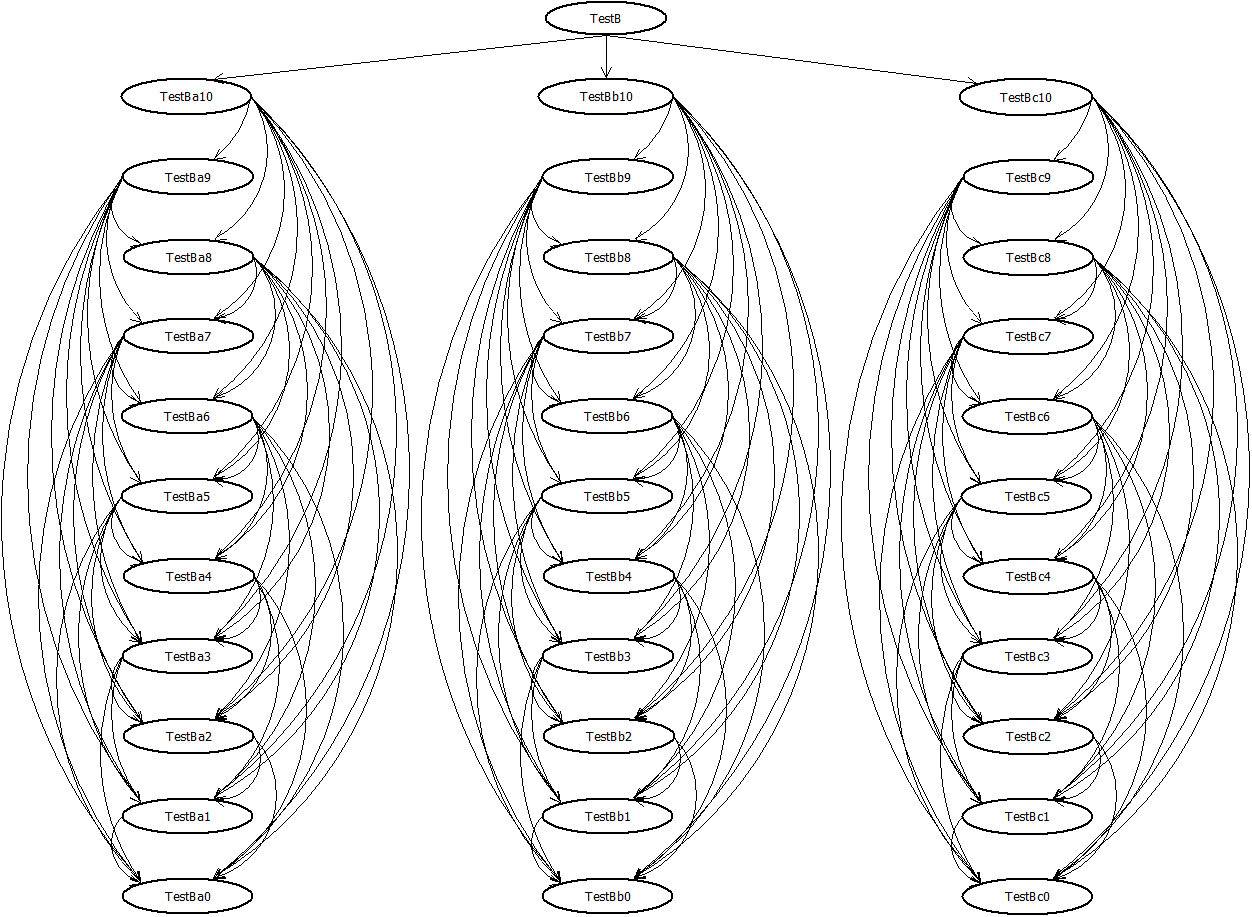
\includegraphics[width=\linewidth]{TestB.png}
  		\caption{Graf zależności dla testu B.}
  		\label{fig:testB}
	\end{center}
\end{figure}

Łatwo wywnioskować, że tworząc obiekty poszczególnych typów liczba tworzonych obiektów rośnie dwukrotnie (tak jak dla testu A):
\begin{itemize}
	\item TestBa0 - 1 obiekt,
	\item TestBa1 - 2 obiekty (obiekt typu TestBa1 i obiekt typu TestBa0),
	\item TestBa2 - 4 obiekty (obiekt typu TestBa2, obiekt typu TestBa1 - 2 obiekty, obiekt typu TestBa0 - 1 obiekt),
	\item TestBa3 - 8 obiektów (obiekt typu TestBa3, obiekt typu TestBa2 - 4 obiekty, obiekt typu TestBa1 - 2 obiekty, obiekt typu TestBa0 - 1 obiekt),
	\item TestBa4 - 16 obiektów,
	\item TestBa5 - 32 obiektów,
	\item TestBa6 - 64 obiektów,
	\item TestBa7 - 128 obiektów,
	\item TestBa8 - 256 obiektów,
	\item TestBa9 - 512 obiektów,
	\item TestBa10 - 1 024 obiektów,
	\item \ldots (dla typów od TestBb0 do TestBb10 i od TestBc0 do TestBc10 sytuacja wygląda dokładnie tak samo jak dla typów od TestBa0 do TestBa10),
	\item TestB - 3 073 obiektów.
\end{itemize}
Zatem tworząc obiekt typu TestB, tworzymy: 1 obiekt typu TestB, 1 obiekt typu TestBa10, TestBb10 i TestBc10, 1 obiekt typu TestBa9, TestBb9 i TestBc9, 2 obiekty typu TestBa8, TestBb8 i TestBc8, 4 obiekty typu TestBa7, TestBb7 i TestBc7, 8 obiektów typu TestBa6, TestBb6 i TestBc6, 16 obiektów typu TestBa5, TestBb5 i TestBc5, 32 obiektów typu TestBa4, TestBb4 i TestBc4, 64 obiektów typu TestBa3, TestBb3 i TestBc3, 128 obiektów typu TestBa2, TestBb2 i TestBc2, 256 obiektów typu TestBa1, TestBb1 i TestBc1, 512 obiektów typu TestBa0, TestBb0 i TestBc0 - co daje w sumie 3 073 obiektów.

\subsubsection{Wyniki Resolve dla Singleton}
\begin{table}[H]
\captionsetup{belowskip=0pt,aboveskip=0pt}
\begin{center}
\begin{small}
	\begin{tabular}{ | l | r r r | }
    		\hline
Liczba & & 1 & \\ \hline
 & min & max & avg \\ \hline
Autofac & 0 & 0 & 0 \\ \hline
Windsor & 0 & 0 & 0 \\ \hline
NiquIoCPartial & 4 & 4 & 4 \\ \hline
SimpleInjector & 6 & 6 & 6 \\ \hline
LightInject & 6 & 7 & 6 \\ \hline
DryIoc & 8 & 8 & 8 \\ \hline
Grace & 8 & 8 & 8 \\ \hline
NiquIoCFull & 8 & 9 & 8 \\ \hline
Ninject & 9 & 10 & 9 \\ \hline
Unity & 23 & 24 & 23 \\ \hline
StructureMap & 32 & 33 & 33 \\ \hline
  	\end{tabular}
\end{small}
\end{center}
\caption{Wyniki testów dla 1 powtórzenia dla operacji Singleton dla Przypadku testowego B}
\label{TestCaseB_Singleton1}
\end{table}
Czasy dla wszystkich rozwiązań wzrosły trzykrotnie w stosunku do przypadku testowego A. Autofac i Windsor poradziły sobie najlepiej, jednakże dopiero dla tego przypadku testowego ich czasy są dużo mniejsze niż pozostałych rozwiązań. Z drugiej strony wyniki dla Unity oraz StructureMap dużo bardziej odstają od reszty.
\\ \\
\begin{table}[H]
\captionsetup{belowskip=0pt,aboveskip=0pt}
\begin{center}
\begin{small}
	\begin{tabular}{ | l | r r r | }
    		\hline
Liczba & & 1000 & \\ \hline
 & min & max & avg \\ \hline
Autofac & 0 & 0 & 0 \\ \hline
Windsor & 0 & 0 & 0 \\ \hline
NiquIoCPartial & 4 & 4 & 4 \\ \hline
SimpleInjector & 6 & 6 & 6 \\ \hline
LightInject & 6 & 7 & 6 \\ \hline
Grace & 8 & 8 & 8 \\ \hline
NiquIoCFull & 8 & 8 & 8 \\ \hline
DryIoc & 8 & 9 & 8 \\ \hline
Ninject & 12 & 13 & 12 \\ \hline
Unity & 24 & 25 & 24 \\ \hline
StructureMap & 33 & 34 & 33 \\ \hline
  	\end{tabular}
\end{small}
\end{center}
\caption{Wyniki testów dla 1000 powtórzeń dla operacji Singleton dla Przypadku testowego B}
\label{TestCaseB_Singleton1000}
\end{table}
Podobnie jak dla przypadku testowego A, tutaj również wraz ze wzrostem liczby powtórzeń nie było znaczącego wzrostu czasu dla żadnego z rozwiązań.

\subsubsection{Wyniki Resolve dla Transient}
\begin{table}[H]
\captionsetup{belowskip=0pt,aboveskip=0pt}
\begin{center}
\begin{small}
	\begin{tabular}{ | l | r r r | }
    		\hline
Liczba & & 1 & \\ \hline
 & min & max & avg \\ \hline
Autofac & 2 & 2 & 2 \\ \hline
NiquIoCPartial & 5 & 5 & 5 \\ \hline
Windsor & 6 & 7 & 6 \\ \hline
NiquIoCFull & 26 & 27 & 26 \\ \hline
Unity & 28 & 29 & 28 \\ \hline
LightInject & 31 & 33 & 32 \\ \hline
StructureMap & 33 & 34 & 33 \\ \hline
Ninject & 36 & 38 & 36 \\ \hline
SimpleInjector & 40 & 41 & 40 \\ \hline
DryIoc & 43 & 44 & 43 \\ \hline
Grace & 50 & 59 & 51 \\ \hline
  	\end{tabular}
\end{small}
\end{center}
\caption{Wyniki testów dla 1 powtórzenia dla operacji Transient dla Przypadku testowego B}
\label{TestCaseB_Transient1}
\end{table}
W tym teście dla 1 powtórzenia Autofac, NiquIoCPartial oraz Windsor zanotowały czasy o rząd wielkości mniejsze niż pozostałe rozwiązania. Dodatkowo najpopularniejsze rozwiązania osiągnęły niższe czasy niż najszybsze rozwiązania.
\\ \\
\begin{table}[H]
\captionsetup{belowskip=0pt,aboveskip=0pt}
\begin{center}
\begin{small}
	\begin{tabular}{ | l | r r r | }
    		\hline
Liczba & & 10 & \\ \hline
 & min & max & avg \\ \hline
NiquIoCPartial & 10 & 10 & 10 \\ \hline
Autofac & 21 & 25 & 21 \\ \hline
NiquIoCFull & 26 & 27 & 26 \\ \hline
LightInject & 32 & 33 & 32 \\ \hline
SimpleInjector & 40 & 42 & 41 \\ \hline
DryIoc & 44 & 45 & 44 \\ \hline
StructureMap & 45 & 46 & 45 \\ \hline
Unity & 49 & 50 & 49 \\ \hline
Windsor & 49 & 69 & 50 \\ \hline
Grace & 51 & 55 & 52 \\ \hline
Ninject & 276 & 337 & 284 \\ \hline
  	\end{tabular}
\end{small}
\end{center}
\caption{Wyniki testów dla 10 powtórzeń dla operacji Transient dla Przypadku testowego B}
\label{TestCaseB_Transient10}
\end{table}
Wraz ze wzrostem liczby powtórzeń wszystkie najpopularniejsze rozwiązania zanotowały wzrost około 10-krotny. NiquIoCPartial zanotował wzrost 2-krotny. NiquIoCFull oraz najszybsze rozwiązania nie zanotowały wzrostu czasów.
\\ \\
\begin{table}[H]
\captionsetup{belowskip=0pt,aboveskip=0pt}
\begin{center}
\begin{small}
	\begin{tabular}{ | l | r r r | }
    		\hline
Liczba & & 100 & \\ \hline
 & min & max & avg \\ \hline
NiquIoCFull & 32 & 33 & 32 \\ \hline
LightInject & 37 & 38 & 37 \\ \hline
SimpleInjector & 47 & 48 & 47 \\ \hline
DryIoc & 51 & 52 & 51 \\ \hline
Grace & 57 & 59 & 58 \\ \hline
NiquIoCPartial & 59 & 79 & 61 \\ \hline
StructureMap & 167 & 175 & 168 \\ \hline
Autofac & 189 & 201 & 191 \\ \hline
Unity & 260 & 271 & 262 \\ \hline
Windsor & 476 & 610 & 484 \\ \hline
Ninject & 2733 & 3595 & 2790 \\ \hline
  	\end{tabular}
\end{small}
\end{center}
\caption{Wyniki testów dla 100 powtórzeń dla operacji Transient dla Przypadku testowego B}
\label{TestCaseB_Transient100}
\end{table}
Gdy liczba powtórzeń wzrosła do 100, to NiquIoCPartial zanotował 5-krotny wzrost. Najpopularniejsze rozwiązania mają stały, około 10-krotny wzrosty. NiquIoCFull oraz wszystkie najszybsze rozwiązania zanotowały nieduży wzrost, jednakże wszystkie poradziły sobie o rząd wielkości lepiej niż najpopularniejsze rozwiązania.
\\ \\
\begin{table}[H]
\captionsetup{belowskip=0pt,aboveskip=0pt}
\begin{center}
\begin{small}
	\begin{tabular}{ | l | r r r | }
    		\hline
Liczba & & 1000 & \\ \hline
 & min & max & avg \\ \hline
NiquIoCFull & 66 & 68 & 66 \\ \hline
LightInject & 70 & 73 & 71 \\ \hline
SimpleInjector & 95 & 97 & 96 \\ \hline
DryIoc & 97 & 100 & 98 \\ \hline
Grace & 122 & 128 & 124 \\ \hline
NiquIoCPartial & 543 & 633 & 550 \\ \hline
StructureMap & 1333 & 1565 & 1346 \\ \hline
Autofac & 1890 & 2044 & 1903 \\ \hline
Unity & 2355 & 2419 & 2366 \\ \hline
Windsor & 4726 & 5665 & 4799 \\ \hline
Ninject & 28220 & 29976 & 28720 \\ \hline
  	\end{tabular}
\end{small}
\end{center}
\caption{Wyniki testów dla 1000 powtórzeń dla operacji Transient dla Przypadku testowego B}
\label{TestCaseB_Transient1000}
\end{table}
NiquIoCFull oraz wszystkie najszybsze rozwiązania zanotowały około 2-krotny wzrost czasów, NiquIoCPartial około 5-krotny, a wszystkie najpopularniejsze rozwiązania utrzymały około 10-krotny wzrost czasów.

\subsubsection{Wyniki Resolve dla TransientSingleton}
\begin{table}[H]
\captionsetup{belowskip=0pt,aboveskip=0pt}
\begin{center}
\begin{small}
	\begin{tabular}{ | l | r r r | }
    		\hline
Liczba & & 1 & \\ \hline
 & min & max & avg \\ \hline
Autofac & 1 & 2 & 1 \\ \hline
Windsor & 3 & 5 & 3 \\ \hline
NiquIoCPartial & 4 & 5 & 5 \\ \hline
NiquIoCFull & 16 & 16 & 16 \\ \hline
Unity & 27 & 28 & 27 \\ \hline
SimpleInjector & 28 & 28 & 28 \\ \hline
Ninject & 29 & 34 & 30 \\ \hline
Grace & 30 & 32 & 31 \\ \hline
StructureMap & 33 & 34 & 33 \\ \hline
LightInject & 48 & 50 & 48 \\ \hline
DryIoc & 56 & 57 & 56 \\ \hline
  	\end{tabular}
\end{small}
\end{center}
\caption{Wyniki testów dla 1 powtórzenia dla operacji TransientSingleton dla Przypadku testowego B}
\label{TestCaseB_TransientSingleton1}
\end{table}
Wyniki dla tego testu są zbliżone do wyników dla Transient. Dla 1 powtórzenia lepiej sobie radzą najpopularniejsze rozwiązania niż te najszybsze. Oba rozwiązania zaprezentowane w tej pracy posiadają czasy zbliżone do najpopularniejszy rozwiązań.
\\ \\
\begin{table}[H]
\captionsetup{belowskip=0pt,aboveskip=0pt}
\begin{center}
\begin{small}
	\begin{tabular}{ | l | r r r | }
    		\hline
Liczba & & 10 & \\ \hline
 & min & max & avg \\ \hline
NiquIoCPartial & 8 & 9 & 8 \\ \hline
NiquIoCFull & 16 & 17 & 16 \\ \hline
Autofac & 18 & 20 & 18 \\ \hline
SimpleInjector & 28 & 29 & 28 \\ \hline
Grace & 31 & 32 & 31 \\ \hline
Windsor & 37 & 46 & 37 \\ \hline
StructureMap & 40 & 46 & 40 \\ \hline
Unity & 46 & 47 & 46 \\ \hline
LightInject & 48 & 50 & 48 \\ \hline
DryIoc & 57 & 58 & 57 \\ \hline
Ninject & 214 & 239 & 219 \\ \hline
  	\end{tabular}
\end{small}
\end{center}
\caption{Wyniki testów dla 10 powtórzeń dla operacji TransientSingleton dla Przypadku testowego B}
\label{TestCaseB_TransientSingleton10}
\end{table}
Dla 10 powtórzeń zarówno NiquIoCPartial jak i NiquIoCFull osiągnęły najmniejsze czasy. Są one jednak zbliżone do pozostały rozwiązań. Wyjątkiem jest jedynie Ninject, który osiągnął czasy o rząd wielkości większe niż reszta.
\\ \\
\begin{table}[H]
\captionsetup{belowskip=0pt,aboveskip=0pt}
\begin{center}
\begin{small}
	\begin{tabular}{ | l | r r r | }
    		\hline
Liczba & & 100 & \\ \hline
 & min & max & avg \\ \hline
NiquIoCFull & 18 & 19 & 18 \\ \hline
SimpleInjector & 32 & 34 & 32 \\ \hline
Grace & 35 & 37 & 35 \\ \hline
NiquIoCPartial & 41 & 57 & 42 \\ \hline
LightInject & 51 & 53 & 51 \\ \hline
DryIoc & 64 & 65 & 64 \\ \hline
StructureMap & 112 & 123 & 113 \\ \hline
Autofac & 172 & 206 & 173 \\ \hline
Unity & 226 & 263 & 228 \\ \hline
Windsor & 355 & 435 & 362 \\ \hline
Ninject & 2013 & 2426 & 2063 \\ \hline
  	\end{tabular}
\end{small}
\end{center}
\caption{Wyniki testów dla 100 powtórzeń dla operacji TransientSingleton dla Przypadku testowego B}
\label{TestCaseB_TransientSingleton100}
\end{table}
Gdy liczba powtórzeń wzrosła do 100, NiquIocFull oraz najszybsze rozwiązania zanotowały niewielki wzrost czasów. Z drugiej strony NiquIocPartial oraz wszystkie najpopularniejsze rozwiązania zanotowały kilkukrotny wzrost.
\\ \\
\begin{table}[H]
\captionsetup{belowskip=0pt,aboveskip=0pt}
\begin{center}
\begin{small}
	\begin{tabular}{ | l | r r r | }
    		\hline
Liczba & & 1000 & \\ \hline
 & min & max & avg \\ \hline
NiquIoCFull & 37 & 39 & 38 \\ \hline
SimpleInjector & 61 & 62 & 61 \\ \hline
Grace & 69 & 72 & 69 \\ \hline
LightInject & 80 & 82 & 80 \\ \hline
DryIoc & 108 & 110 & 109 \\ \hline
NiquIoCPartial & 365 & 406 & 368 \\ \hline
StructureMap & 797 & 915 & 805 \\ \hline
Autofac & 1698 & 1832 & 1709 \\ \hline
Unity & 2016 & 2305 & 2032 \\ \hline
Windsor & 3543 & 4824 & 3637 \\ \hline
Ninject & 20440 & 22891 & 20858 \\ \hline
  	\end{tabular}
\end{small}
\end{center}
\caption{Wyniki testów dla 1000 powtórzeń dla operacji TransientSingleton dla Przypadku testowego B}
\label{TestCaseB_TransientSingleton1000}
\end{table}
Podobnie jak dla testu dla Transient, NiquIocPartial i najpopularniejsze rozwiązania utrzymały liniowy, około 10-krotny wzrosty. Dla pozostałych rozwiązań ten wzrost był około 2-krotny.

\subsubsection{Wyniki Resolve dla PerThread}
\begin{table}[H]
\captionsetup{belowskip=0pt,aboveskip=0pt}
\begin{center}
\begin{small}
	\begin{tabular}{ | l | r r r | }
    		\hline
Liczba & & 1 & \\ \hline
 & min & max & avg \\ \hline
Autofac & 0 & 0 & 0 \\ \hline
Windsor & 0 & 0 & 0 \\ \hline
NiquIoCPartial & 4 & 5 & 4 \\ \hline
NiquIoCFull & 8 & 8 & 8 \\ \hline
Ninject & 9 & 10 & 9 \\ \hline
Grace & 13 & 13 & 13 \\ \hline
SimpleInjector & 23 & 23 & 23 \\ \hline
Unity & 23 & 25 & 23 \\ \hline
StructureMap & 32 & 34 & 33 \\ \hline
DryIoc & 246 & 250 & 247 \\ \hline
LightInject & 409 & 419 & 412 \\ \hline
  	\end{tabular}
\end{small}
\end{center}
\caption{Wyniki testów dla 1 powtórzenia dla operacji PerThread dla Przypadku testowego B}
\label{TestCaseB_PerThread1}
\end{table}
Dla tego testu sytuacja wygląda identycznie jak dla przypadku testowego A - DryIoc oraz LightInject nie poradziły sobie z rejestracją PerThread i zanotowały czas o rząd wielkości większe niż pozostałe rozwiązania.\\
\\
Wyraźnie najlepiej poradziły sobie Autofac i Windsor, a dalej NiquIoCPartial oraz NiquIoCFull. Czasy niedużo większe osiągnęły również Ninject, a także Grace.
\\ \\
\begin{table}[H]
\captionsetup{belowskip=0pt,aboveskip=0pt}
\begin{center}
\begin{small}
	\begin{tabular}{ | l | r r r | }
    		\hline
Liczba & & 1000 & \\ \hline
 & min & max & avg \\ \hline
Autofac & 0 & 0 & 0 \\ \hline
Windsor & 0 & 0 & 0 \\ \hline
NiquIoCPartial & 4 & 5 & 4 \\ \hline
NiquIoCFull & 8 & 8 & 8 \\ \hline
Ninject & 12 & 13 & 13 \\ \hline
Grace & 13 & 14 & 13 \\ \hline
SimpleInjector & 23 & 24 & 23 \\ \hline
Unity & 24 & 25 & 24 \\ \hline
StructureMap & 33 & 34 & 33 \\ \hline
DryIoc & 246 & 249 & 247 \\ \hline
LightInject & 409 & 420 & 413 \\ \hline
  	\end{tabular}
\end{small}
\end{center}
\caption{Wyniki testów dla 1000 powtórzeń dla operacji PerThread dla Przypadku testowego B}
\label{TestCaseB_PerThread1000}
\end{table}
Gdy liczba powtórzeń wzrosła do 1000 żadne z rozwiązań nie zanotowało wzrostu czasów.

\subsubsection{Wyniki Resolve dla FactoryMethod}
\begin{table}[H]
\captionsetup{belowskip=0pt,aboveskip=0pt}
\begin{center}
\begin{small}
	\begin{tabular}{ | l | r r r | }
    		\hline
Liczba & & 1 & \\ \hline
 & min & max & avg \\ \hline
DryIoc & 0 & 0 & 0 \\ \hline
NiquIoCPartial & 0 & 0 & 0 \\ \hline
NiquIoCFull & 0 & 0 & 0 \\ \hline
Autofac & 1 & 1 & 1 \\ \hline
LightInject & 2 & 4 & 2 \\ \hline
SimpleInjector & 4 & 4 & 4 \\ \hline
Windsor & 4 & 5 & 4 \\ \hline
Unity & 4 & 6 & 4 \\ \hline
Grace & 7 & 9 & 7 \\ \hline
Ninject & 23 & 25 & 24 \\ \hline
StructureMap & 25 & 25 & 25 \\ \hline
  	\end{tabular}
\end{small}
\end{center}
\caption{Wyniki testów dla 1 powtórzenia dla operacji FactoryMethod dla Przypadku testowego B}
\label{TestCaseB_FactoryMethod1}
\end{table}
Dla 1 powtórzenia wszystkie rozwiązania za wyjątkiem Ninject i StructureMap mają zbliżone, nieduże czasy. Te dwa rozwiązania zanotowały czasy o rząd wielkości większe niż pozostałe.
\\
\begin{table}[H]
\captionsetup{belowskip=0pt,aboveskip=0pt}
\begin{center}
\begin{small}
	\begin{tabular}{ | l | r r r | }
    		\hline
Liczba & & 10 & \\ \hline
 & min & max & avg \\ \hline
DryIoc & 1 & 2 & 1 \\ \hline
NiquIoCFull & 3 & 4 & 3 \\ \hline
LightInject & 4 & 4 & 4 \\ \hline
NiquIoCPartial & 4 & 4 & 4 \\ \hline
SimpleInjector & 7 & 7 & 7 \\ \hline
Grace & 10 & 10 & 10 \\ \hline
Autofac & 16 & 17 & 16 \\ \hline
Windsor & 33 & 36 & 33 \\ \hline
StructureMap & 37 & 37 & 37 \\ \hline
Unity & 44 & 45 & 44 \\ \hline
Ninject & 166 & 182 & 170 \\ \hline
  	\end{tabular}
\end{small}
\end{center}
\caption{Wyniki testów dla 10 powtórzeń dla operacji FactoryMethod dla Przypadku testowego B}
\label{TestCaseB_FactoryMethod10}
\end{table}
Najszybsze rozwiązania zanotowały około 2-krotny wzrost czasów, a z kolei dla NiquIoCPartial oraz najpopularniejszych rozwiązań ten wzrost było około 10-krotny. NiquIoCFull osiągnął kilkukrotny wzrost czasów, ale poradził sobie słabiej tylko od DryIoc.
\\ \\
\begin{table}[H]
\captionsetup{belowskip=0pt,aboveskip=0pt}
\begin{center}
\begin{small}
	\begin{tabular}{ | l | r r r | }
    		\hline
Liczba & & 100 & \\ \hline
 & min & max & avg \\ \hline
DryIoc & 19 & 19 & 19 \\ \hline
LightInject & 21 & 22 & 21 \\ \hline
NiquIoCFull & 35 & 37 & 35 \\ \hline
SimpleInjector & 35 & 37 & 36 \\ \hline
NiquIoCPartial & 37 & 39 & 38 \\ \hline
Grace & 38 & 39 & 39 \\ \hline
Autofac & 154 & 156 & 155 \\ \hline
StructureMap & 159 & 162 & 160 \\ \hline
Windsor & 298 & 321 & 301 \\ \hline
Unity & 436 & 443 & 439 \\ \hline
Ninject & 1601 & 1670 & 1622 \\ \hline
  	\end{tabular}
\end{small}
\end{center}
\caption{Wyniki testów dla 100 powtórzeń dla operacji FactoryMethod dla Przypadku testowego B}
\label{TestCaseB_FactoryMethod100}
\end{table}
Wraz ze wzrostem powtórzeń do 100, większość rozwiązań zanotowała około 10-krotny wzrost czasów. Wyjątkami są LightInject, SimpleInjector, Grace i StructureMap, które zanotował około 5-krotny wzrost czasów.
\\ \\
\begin{table}[H]
\captionsetup{belowskip=0pt,aboveskip=0pt}
\begin{center}
\begin{small}
	\begin{tabular}{ | l | r r r | }
    		\hline
Liczba & & 1000 & \\ \hline
 & min & max & avg \\ \hline
LightInject & 180 & 186 & 182 \\ \hline
DryIoc & 185 & 188 & 186 \\ \hline
SimpleInjector & 305 & 311 & 308 \\ \hline
Grace & 312 & 319 & 315 \\ \hline
NiquIoCFull & 344 & 373 & 353 \\ \hline
NiquIoCPartial & 364 & 373 & 368 \\ \hline
StructureMap & 1347 & 1385 & 1359 \\ \hline
Autofac & 1545 & 1573 & 1550 \\ \hline
Windsor & 2939 & 3226 & 2971 \\ \hline
Unity & 4355 & 4492 & 4373 \\ \hline
Ninject & 16788 & 17602 & 16963 \\ \hline
  	\end{tabular}
\end{small}
\end{center}
\caption{Wyniki testów dla 1000 powtórzeń dla operacji FactoryMethod dla Przypadku testowego B}
\label{TestCaseB_FactoryMethod1000}
\end{table}
Gdy liczba powtórzeń wzrosła do 1000, to wszystkie rozwiązania zanotowały około 9-krotny lub 10-krotny wzrost. Najmniejsze czasy zanotowały LightInject oraz DryIoC.


\subsection{Przypadek testowy C}
\subsubsection{Opis}
Ten przypadek testowy znacząco różni się od dwóch poprzednich. Mamy tutaj zdefiniowanych 26 typów. 5 z tych typów ma konstruktor bezparametrowy, a pozostałe 21 ma konstruktor z pięcioma parametrami. Typem głównym jest typ "TestC". Obiekt tego typy w konstruktorze przyjmuje 5 obiektów, kolejno następujących typów: "TestC40", "TestC41", "TestC42", "TestC43" i "TestC44". Każdy z tych pięciu typów ma taki sam konstruktor - przyjmuje w nim 5 obiektów o typach, które w nazwie mają pierwszą cyfrę o 1 mniejszą, czyli są to obiekty typów od "TestC30" do "TestC34". Dla tych i kolejnych typów zasada z konstruktorami wygląda tak samo. Na końcu dochodzimy do typów od "TestC00" do "TestC04", które mają konstruktor bezparametrowy. Rys. \ref{fig:testC} przedstawia graf zależności typów dla tego przypadku testowego.\\
\begin{figure}[H]
	\begin{center}
  		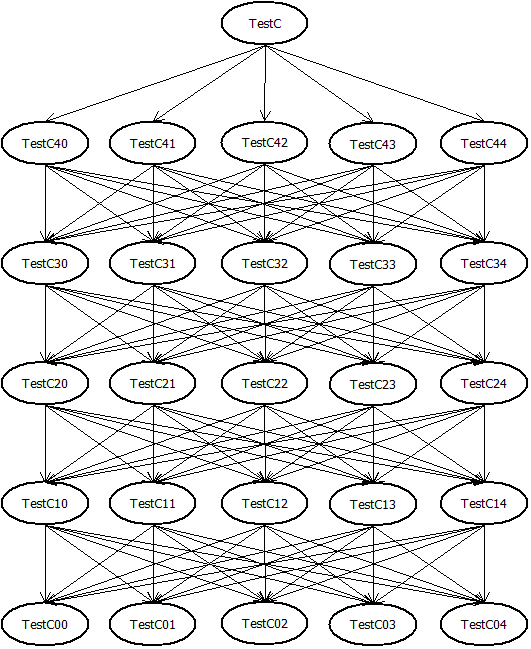
\includegraphics[height=11.5cm]{TestC.png}
  		\caption{Graf zależności dla testu C.}
  		\label{fig:testC}
	\end{center}
\end{figure}

Łatwo wywnioskować, że tworząc obiekty poszczególnych typów liczba tworzonych obiektów rośnie ponad pięciokrotnie:
\begin{itemize}
	\item typy od TestC00 do TestC04 - 1 obiekt,
	\item typy od TestC10 do TestC14 - 6 obiektów (obiekt danego typu plus 5 obiektów typów od TestC00 do TestC04),
	\item typy od TestC20 do TestC24 - 31 obiektów (obiekt danego typu plus 5 obiektów typów od TestC10 do TestC14),
	\item typy od TestC30 do TestC34 - 156 obiektów,
	\item  typy od TestC40 do TestC44 - 781 obiektów,
	\item TestC - 3 906 obiektów.
\end{itemize}
Zatem tworząc obiekt typu TestC, tworzymy: 1 obiekt typu TestC, 5 obiektów typów od TestC40 do TestC44, 25 obiektów typów od TestC30 do TestC34, 125 obiektów typów od TestC20 do TestC24, 625 obiektów typów od TestC10 do TestC14 oraz 3 125 obiektów typów od TestC00 do TestC04 - co daje w sumie 3 906 obiektów.

\subsubsection{Wyniki Resolve dla Singleton}
\begin{table}[H]
\captionsetup{belowskip=0pt,aboveskip=0pt}
\begin{center}
\begin{small}
	\begin{tabular}{ | l | r r r | }
    		\hline
Liczba & & 1 & \\ \hline
 & min & max & avg \\ \hline
Autofac & 0 & 0 & 0 \\ \hline
Windsor & 0 & 0 & 0 \\ \hline
NiquIoCPartial & 3 & 3 & 3 \\ \hline
LightInject & 4 & 4 & 4 \\ \hline
SimpleInjector & 4 & 4 & 4 \\ \hline
DryIoc & 5 & 5 & 5 \\ \hline
Grace & 5 & 5 & 5 \\ \hline
NiquIoCFull & 5 & 5 & 5 \\ \hline
Ninject & 6 & 6 & 6 \\ \hline
Unity & 15 & 16 & 15 \\ \hline
StructureMap & 22 & 23 & 22 \\ \hline
  	\end{tabular}
\end{small}
\end{center}
\caption{Wyniki testów dla 1 powtórzenia dla operacji Singleton dla Przypadku testowego C}
\label{TestCaseC_Singleton1}
\end{table}
Najlepiej poradził sobie Autofac i Windsor, a najsłabiej Unity oraz StructureMap. Pozostałe rozwiązania zanotowały zbliżone czasy.
\\ \\
\begin{table}[H]
\captionsetup{belowskip=0pt,aboveskip=0pt}
\begin{center}
\begin{small}
	\begin{tabular}{ | l | r r r | }
    		\hline
Liczba & & 1000 & \\ \hline
 & min & max & avg \\ \hline
Autofac & 0 & 0 & 0 \\ \hline
Windsor & 0 & 0 & 0 \\ \hline
NiquIoCPartial & 3 & 3 & 3 \\ \hline
LightInject & 4 & 4 & 4 \\ \hline
SimpleInjector & 4 & 4 & 4 \\ \hline
DryIoc & 5 & 5 & 5 \\ \hline
Grace & 5 & 5 & 5 \\ \hline
NiquIoCFull & 5 & 5 & 5 \\ \hline
Ninject & 9 & 10 & 9 \\ \hline
Unity & 16 & 17 & 16 \\ \hline
StructureMap & 23 & 24 & 23 \\ \hline
  	\end{tabular}
\end{small}
\end{center}
\caption{Wyniki testów dla 1000 powtórzeń dla operacji Singleton dla Przypadku testowego C}
\label{TestCaseC_Singleton1000}
\end{table}
Dla tego przypadku testowego sytuacja dla tego testu wygląda identycznie jak dla dwóch poprzednich przypadków testowych. Wraz ze wzrostem powtórzeń, czasy pozostają na tym samym poziomie, a tabela z wynikami jest zbliżona do tabeli dla przypadku testowego A i B.

\subsubsection{Wyniki Resolve dla Transient}
\begin{table}[H]
\captionsetup{belowskip=0pt,aboveskip=0pt}
\begin{center}
\begin{small}
	\begin{tabular}{ | l | r r r | }
    		\hline
Liczba & & 1 & \\ \hline
 & min & max & avg \\ \hline
Autofac & 2 & 2 & 2 \\ \hline
NiquIoCPartial & 3 & 4 & 4 \\ \hline
Windsor & 7 & 8 & 7 \\ \hline
Unity & 18 & 19 & 19 \\ \hline
StructureMap & 26 & 27 & 26 \\ \hline
NiquIoCFull & 31 & 33 & 31 \\ \hline
LightInject & 36 & 37 & 36 \\ \hline
DryIoc & 39 & 41 & 39 \\ \hline
Ninject & 38 & 42 & 39 \\ \hline
SimpleInjector & 40 & 42 & 41 \\ \hline
Grace & 61 & 63 & 61 \\ \hline
  	\end{tabular}
\end{small}
\end{center}
\caption{Wyniki testów dla 1 powtórzenia dla operacji Transient dla Przypadku testowego C}
\label{TestCaseC_Transient1}
\end{table}
Dla 1 powtórzenia najlepiej radzą sobie najpopularniejsze rozwiązania oraz NiquIoCPartial. Dalej jest NiquIoCFull, a za nim wszystkie najszybsze rozwiązania. Najniższe czasy osiągnęły Autofac i NiquIoCPartial.
\\ \\
\begin{table}[H]
\captionsetup{belowskip=0pt,aboveskip=0pt}
\begin{center}
\begin{small}
	\begin{tabular}{ | l | r r r | }
    		\hline
Liczba & & 10 & \\ \hline
 & min & max & avg \\ \hline
NiquIoCPartial & 10 & 11 & 10 \\ \hline
Autofac & 23 & 25 & 24 \\ \hline
NiquIoCFull & 31 & 33 & 32 \\ \hline
LightInject & 36 & 39 & 37 \\ \hline
DryIoc & 40 & 41 & 40 \\ \hline
StructureMap & 40 & 42 & 40 \\ \hline
SimpleInjector & 41 & 43 & 41 \\ \hline
Unity & 47 & 51 & 47 \\ \hline
Grace & 62 & 65 & 62 \\ \hline
Windsor & 61 & 82 & 62 \\ \hline
Ninject & 345 & 375 & 353 \\ \hline
  	\end{tabular}
\end{small}
\end{center}
\caption{Wyniki testów dla 10 powtórzeń dla operacji Transient dla Przypadku testowego C}
\label{TestCaseC_Transient10}
\end{table}
Tym razem również wszystkie najpopularniejsze rozwiązania zanotowały około 10-krotny wzrost, NiquIoCPartial około 2-krotny wzrost, a NiquIoCFull oraz wszystkie najszybsze rozwiązania osiągnęły podobne czasy co dla 1 powtórzenia.
\\ \\
\begin{table}[H]
\captionsetup{belowskip=0pt,aboveskip=0pt}
\begin{center}
\begin{small}
	\begin{tabular}{ | l | r r r | }
    		\hline
Liczba & & 100 & \\ \hline
 & min & max & avg \\ \hline
NiquIoCFull & 38 & 41 & 38 \\ \hline
LightInject & 43 & 49 & 44 \\ \hline
DryIoc & 47 & 48 & 47 \\ \hline
SimpleInjector & 49 & 51 & 49 \\ \hline
Grace & 73 & 74 & 73 \\ \hline
NiquIoCPartial & 72 & 80 & 74 \\ \hline
StructureMap & 178 & 207 & 181 \\ \hline
Autofac & 229 & 250 & 231 \\ \hline
Unity & 315 & 369 & 318 \\ \hline
Windsor & 594 & 769 & 608 \\ \hline
Ninject & 3430 & 4043 & 3511 \\ \hline
  	\end{tabular}
\end{small}
\end{center}
\caption{Wyniki testów dla 100 powtórzeń dla operacji Transient dla Przypadku testowego C}
\label{TestCaseC_Transient100}
\end{table}
Pomimo że ten przypadek testowy znacząco różni się od poprzednich dwóch, to stosunek wzrostów czasów, wraz ze wzrostem powtórzeń dla tego testu wydaje się być taki sam. NiquIoCFull oraz najszybsze rozwiązania notują niewielki wzrost i ich czasy są na tym samym poziomie co dla 10 powtórzeń, a pozostałe rozwiązania mają wyniki około 9-10 razy większe.
\\ \\
\begin{table}[H]
\captionsetup{belowskip=0pt,aboveskip=0pt}
\begin{center}
\begin{small}
	\begin{tabular}{ | l | r r r | }
    		\hline
Liczba & & 1000 & \\ \hline
 & min & max & avg \\ \hline
NiquIoCFull & 81 & 83 & 82 \\ \hline
LightInject & 86 & 88 & 86 \\ \hline
DryIoc & 98 & 100 & 99 \\ \hline
SimpleInjector & 115 & 117 & 116 \\ \hline
Grace & 153 & 163 & 155 \\ \hline
NiquIoCPartial & 683 & 781 & 690 \\ \hline
StructureMap & 1520 & 1810 & 1540 \\ \hline
Autofac & 2274 & 2419 & 2288 \\ \hline
Unity & 2995 & 3359 & 3015 \\ \hline
Windsor & 5898 & 7708 & 6037 \\ \hline
Ninject & 36072 & 42914 & 37642 \\ \hline
  	\end{tabular}
\end{small}
\end{center}
\caption{Wyniki testów dla 1000 powtórzeń dla operacji Transient dla Przypadku testowego C}
\label{TestCaseC_Transient1000}
\end{table}
Tendencja wzrostów się utrzymała i NiquIoCFull radzi sobie lepiej niż wszystkie najszybsze rozwiązania, a NiquIoCPartial niż wszystkie najpopularniejsze rozwiązania.

\subsubsection{Wyniki Resolve dla TransientSingleton}
\begin{table}[H]
\captionsetup{belowskip=0pt,aboveskip=0pt}
\begin{center}
\begin{small}
	\begin{tabular}{ | l | r r r | }
    		\hline
Liczba & & 1 & \\ \hline
 & min & max & avg \\ \hline
Autofac & 1 & 2 & 2 \\ \hline
NiquIoCPartial & 3 & 3 & 3 \\ \hline
Windsor & 3 & 3 & 3 \\ \hline
NiquIoCFull & 12 & 13 & 12 \\ \hline
Unity & 18 & 18 & 18 \\ \hline
SimpleInjector & 21 & 22 & 21 \\ \hline
StructureMap & 23 & 23 & 23 \\ \hline
Grace & 23 & 24 & 23 \\ \hline
Ninject & 25 & 30 & 26 \\ \hline
LightInject & 52 & 54 & 52 \\ \hline
DryIoc & 58 & 70 & 58 \\ \hline
  	\end{tabular}
\end{small}
\end{center}
\caption{Wyniki testów dla 1 powtórzenia dla operacji TransientSingleton dla Przypadku testowego C}
\label{TestCaseC_TransientSingleton1}
\end{table}
Dla 1 powtórzenia najlepiej radzą sobie Autofac, NiquIoCPartial i Windsor. Pozostałe rozwiązania zanotowały czasy od kilku, do kilkunastu razy większe. Najsłabiej poradziły sobie LightInject oraz DryIoc.
\\ \\
\begin{table}[H]
\captionsetup{belowskip=0pt,aboveskip=0pt}
\begin{center}
\begin{small}
	\begin{tabular}{ | l | r r r | }
    		\hline
Liczba & & 10 & \\ \hline
 & min & max & avg \\ \hline
NiquIoCPartial & 6 & 7 & 6 \\ \hline
NiquIoCFull & 12 & 13 & 12 \\ \hline
Autofac & 19 & 20 & 20 \\ \hline
SimpleInjector & 21 & 22 & 21 \\ \hline
Grace & 23 & 24 & 23 \\ \hline
StructureMap & 30 & 31 & 30 \\ \hline
Windsor & 34 & 41 & 35 \\ \hline
Unity & 39 & 41 & 40 \\ \hline
LightInject & 52 & 55 & 53 \\ \hline
DryIoc & 59 & 62 & 59 \\ \hline
Ninject & 199 & 231 & 203 \\ \hline
  	\end{tabular}
\end{small}
\end{center}
\caption{Wyniki testów dla 10 powtórzeń dla operacji TransientSingleton dla Przypadku testowego C}
\label{TestCaseC_TransientSingleton10}
\end{table}
Gdy mamy 10 powtórzeń zarówno NiquIoCFull jak i wszystkie najszybsze rozwiązania nie zanotowały wzrostu czasów. NiquIoCPartial, Unity oraz StructureMap zanotowały wzrost około 2-krotny, a Autofac, Windsor oraz Ninject około 10-krotny. Mimo że dla LightInject i DryIoC czasy nie wzrosły, to i tak dla tylu powtórzeń osiągnęły one jedne z najwyższych wyników.
\\ \\
\begin{table}[H]
\captionsetup{belowskip=0pt,aboveskip=0pt}
\begin{center}
\begin{small}
	\begin{tabular}{ | l | r r r | }
    		\hline
Liczba & & 100 & \\ \hline
 & min & max & avg \\ \hline
NiquIoCFull & 13 & 14 & 14 \\ \hline
SimpleInjector & 23 & 24 & 24 \\ \hline
Grace & 25 & 26 & 25 \\ \hline
NiquIoCPartial & 38 & 46 & 39 \\ \hline
LightInject & 55 & 57 & 56 \\ \hline
DryIoc & 65 & 68 & 65 \\ \hline
StructureMap & 80 & 84 & 80 \\ \hline
Autofac & 184 & 198 & 187 \\ \hline
Unity & 242 & 258 & 243 \\ \hline
Windsor & 338 & 400 & 343 \\ \hline
Ninject & 1903 & 2364 & 1951 \\ \hline
  	\end{tabular}
\end{small}
\end{center}
\caption{Wyniki testów dla 100 powtórzeń dla operacji TransientSingleton dla Przypadku testowego C}
\label{TestCaseC_TransientSingleton100}
\end{table}
Przy 100 powtórzeniach wzrost czasów wygląda identycznie jak dla testu Transient - NiquIoCFull oraz najszybsze rozwiązania mają niewielki, a pozostałe rozwiązania kilkukrotny. LightInject i DryIoC tym razem zanotowały czasy lepsze niż wszystkie najpopularniejsze rozwiążania, ale wciąż słabsze niż NiquIoCPartial.
\\ \\
\begin{table}[H]
\captionsetup{belowskip=0pt,aboveskip=0pt}
\begin{center}
\begin{small}
	\begin{tabular}{ | l | r r r | }
    		\hline
Liczba & & 1000 & \\ \hline
 & min & max & avg \\ \hline
NiquIoCFull & 25 & 26 & 25 \\ \hline
Grace & 44 & 45 & 44 \\ \hline
SimpleInjector & 44 & 45 & 44 \\ \hline
LightInject & 82 & 85 & 83 \\ \hline
DryIoc & 105 & 107 & 106 \\ \hline
NiquIoCPartial & 347 & 359 & 349 \\ \hline
StructureMap & 549 & 593 & 553 \\ \hline
Autofac & 1810 & 1898 & 1831 \\ \hline
Unity & 2258 & 2428 & 2272 \\ \hline
Windsor & 3368 & 4115 & 3429 \\ \hline
Ninject & 19137 & 22595 & 19626 \\ \hline
  	\end{tabular}
\end{small}
\end{center}
\caption{Wyniki testów dla 1000 powtórzeń dla operacji TransientSingleton dla Przypadku testowego C}
\label{TestCaseC_TransientSingleton1000}
\end{table}
Dla 1000 powtórzeń najmniejszy czas zanotował NiquIoCFull, a dalej wszystkie najszybsze rozwiązania. NiquIoCPartial dla tego przypadku testowego również znalazł się za wszystkimi najszybszymi rozwiązaniami oraz przed wszystkimi najpopularniejszymi rozwiązaniami.

\subsubsection{Wyniki Resolve dla PerThread}
\begin{table}[H]
\captionsetup{belowskip=0pt,aboveskip=0pt}
\begin{center}
\begin{small}
	\begin{tabular}{ | l | r r r | }
    		\hline
Liczba & & 1 & \\ \hline
 & min & max & avg \\ \hline
Autofac & 0 & 0 & 0 \\ \hline
Windsor & 0 & 0 & 0 \\ \hline
NiquIoCPartial & 3 & 3 & 3 \\ \hline
NiquIoCFull & 5 & 5 & 5 \\ \hline
Ninject & 6 & 7 & 6 \\ \hline
Grace & 8 & 9 & 8 \\ \hline
Unity & 15 & 16 & 15 \\ \hline
SimpleInjector & 16 & 16 & 16 \\ \hline
StructureMap & 22 & 23 & 22 \\ \hline
DryIoc & 157 & 162 & 158 \\ \hline
LightInject & 525 & 556 & 529 \\ \hline
  	\end{tabular}
\end{small}
\end{center}
\caption{Wyniki testów dla 1 powtórzenia dla operacji PerThread dla Przypadku testowego C}
\label{TestCaseC_PerThread1}
\end{table}
Dla tego przypadku testowego wyniki są podobne jak w poprzednich przypadkach testowych - najlepiej poradziły sobie Autofac i Windsor, następnie dwa rozwiązania zaprezentowane w tej pracy, a dalej pozostałe rozwiązania. Najsłabsze czasy uzyskały DryIoc oraz LightInject, które nie radzą sobie z rejestracją PerThread.
\\ \\
\begin{table}[H]
\captionsetup{belowskip=0pt,aboveskip=0pt}
\begin{center}
\begin{small}
	\begin{tabular}{ | l | r r r | }
    		\hline
Liczba & & 1000 & \\ \hline
 & min & max & avg \\ \hline
Autofac & 0 & 0 & 0 \\ \hline
Windsor & 0 & 0 & 0 \\ \hline
NiquIoCPartial & 3 & 3 & 3 \\ \hline
NiquIoCFull & 5 & 5 & 5 \\ \hline
Grace & 8 & 9 & 8 \\ \hline
Ninject & 9 & 10 & 9 \\ \hline
Unity & 16 & 17 & 16 \\ \hline
SimpleInjector & 16 & 18 & 16 \\ \hline
StructureMap & 23 & 73 & 24 \\ \hline
DryIoc & 158 & 161 & 158 \\ \hline
LightInject & 525 & 550 & 529 \\ \hline
  	\end{tabular}
\end{small}
\end{center}
\caption{Wyniki testów dla 1000 powtórzeń dla operacji PerThread dla Przypadku testowego C}
\label{TestCaseC_PerThread1000}
\end{table}
Test dla 1000 powtórzeń pokazał, że dla żadnego rozwiązania wraz ze wzrostem liczby powtórzeń, dla tego testu nie wzrasta czas.

\subsubsection{Wyniki Resolve dla FactoryMethod}
\begin{table}[H]
\captionsetup{belowskip=0pt,aboveskip=0pt}
\begin{center}
\begin{small}
	\begin{tabular}{ | l | r r r | }
    		\hline
Liczba & & 1 & \\ \hline
 & min & max & avg \\ \hline
DryIoc & 0 & 0 & 0 \\ \hline
NiquIoCPartial & 0 & 0 & 0 \\ \hline
NiquIoCFull & 0 & 0 & 0 \\ \hline
Autofac & 2 & 2 & 2 \\ \hline
LightInject & 2 & 2 & 2 \\ \hline
SimpleInjector & 3 & 4 & 3 \\ \hline
Windsor & 4 & 5 & 4 \\ \hline
Grace & 6 & 6 & 6 \\ \hline
Unity & 6 & 7 & 6 \\ \hline
StructureMap & 18 & 20 & 18 \\ \hline
Ninject & 26 & 28 & 27 \\ \hline
  	\end{tabular}
\end{small}
\end{center}
\caption{Wyniki testów dla 1 powtórzenia dla operacji FactoryMethod dla Przypadku testowego C}
\label{TestCaseC_FactoryMethod1}
\end{table}
Gdy mamy 1 powtórzenie najlepiej radzą sobie NiquIoCPartial, NiquIoCFull oraz najszybsze rozwiązania. Najpopularniejsze rozwiązania zanotowały czasy trochę (Autofac, Windsor, Unity) lub dużo (StructureMap, Ninject) słabsze.
\\ \\
\begin{table}[H]
\captionsetup{belowskip=0pt,aboveskip=0pt}
\begin{center}
\begin{small}
	\begin{tabular}{ | l | r r r | }
    		\hline
Liczba & & 10 & \\ \hline
 & min & max & avg \\ \hline
DryIoc & 2 & 2 & 2 \\ \hline
NiquIoCFull & 4 & 4 & 4 \\ \hline
LightInject & 4 & 5 & 4 \\ \hline
NiquIoCPartial & 5 & 5 & 5 \\ \hline
SimpleInjector & 7 & 7 & 7 \\ \hline
Grace & 9 & 9 & 9 \\ \hline
Autofac & 19 & 21 & 19 \\ \hline
StructureMap & 34 & 35 & 34 \\ \hline
Windsor & 38 & 41 & 39 \\ \hline
Unity & 56 & 58 & 56 \\ \hline
Ninject & 209 & 220 & 213 \\ \hline
  	\end{tabular}
\end{small}
\end{center}
\caption{Wyniki testów dla 10 powtórzeń dla operacji FactoryMethod dla Przypadku testowego C}
\label{TestCaseC_FactoryMethod10}
\end{table}
Wraz ze wzrostem liczby powtórzeń, czasy dla wszystkich rozwiązań wzrosły - dla rozwiązań najszybszych był to wzrost około 2-krotny, a dla pozostałych około 10-krotny.
\\ \\
\begin{table}[H]
\captionsetup{belowskip=0pt,aboveskip=0pt}
\begin{center}
\begin{small}
	\begin{tabular}{ | l | r r r | }
    		\hline
Liczba & & 100 & \\ \hline
 & min & max & avg \\ \hline
DryIoc & 24 & 25 & 24 \\ \hline
LightInject & 24 & 27 & 25 \\ \hline
Grace & 42 & 44 & 42 \\ \hline
NiquIoCFull & 42 & 45 & 43 \\ \hline
SimpleInjector & 43 & 45 & 44 \\ \hline
NiquIoCPartial & 45 & 47 & 46 \\ \hline
StructureMap & 177 & 198 & 180 \\ \hline
Autofac & 186 & 197 & 189 \\ \hline
Windsor & 366 & 378 & 369 \\ \hline
Unity & 555 & 645 & 564 \\ \hline
Ninject & 2110 & 2474 & 2152 \\ \hline
  	\end{tabular}
\end{small}
\end{center}
\caption{Wyniki testów dla 100 powtórzeń dla operacji FactoryMethod dla Przypadku testowego C}
\label{TestCaseC_FactoryMethod100}
\end{table}
Gdy mamy 100 powtórzeń wyraźnie wyższe czasy osiągnęły najpopularniejsze rozwiązania. Najniższe czasy zanotowały DryIoC oraz LightInject, a pozostałe rozwiązania (Grace, NiquIoCFull, SimpleInjector i NiquIoCPartial) uzyskały podobne wyniki.
\\ \\
\begin{table}[H]
\captionsetup{belowskip=0pt,aboveskip=0pt}
\begin{center}
\begin{small}
	\begin{tabular}{ | l | r r r | }
    		\hline
Liczba & & 1000 & \\ \hline
 & min & max & avg \\ \hline
LightInject & 215 & 223 & 218 \\ \hline
DryIoc & 232 & 236 & 234 \\ \hline
Grace & 357 & 369 & 361 \\ \hline
SimpleInjector & 380 & 389 & 385 \\ \hline
NiquIoCFull & 419 & 440 & 424 \\ \hline
NiquIoCPartial & 446 & 479 & 451 \\ \hline
StructureMap & 1594 & 1748 & 1623 \\ \hline
Autofac & 1867 & 1979 & 1880 \\ \hline
Windsor & 3650 & 4077 & 3721 \\ \hline
Unity & 5561 & 5645 & 5577 \\ \hline
Ninject & 22141 & 23030 & 22398 \\ \hline
  	\end{tabular}
\end{small}
\end{center}
\caption{Wyniki testów dla 1000 powtórzeń dla operacji FactoryMethod dla Przypadku testowego C}
\label{TestCaseC_FactoryMethod1000}
\end{table}
Przy 1000 powtórzeniach wszystkie rozwiązania zanotowały liniowy, około 10-krotny wzrost. Jednakże najmniejszy przyrost czasu zanotował LightInject i to on osiągnął najlepszy czas.


\subsection{Przypadek testowy D}
\subsubsection{Opis}
Podobnie jak przypadek testowy B jest analogiczny z przypadkiem A, tak ten przypadek, jest zbliżony do przypadku C. Mamy tutaj tyle samo poziomów, co dla C, ale na każdym poziomie (poza pierwszym) obiektów jest dwa razy więcej. Zatem w tym teście mamy zdefiniowanych 51 typów. Tutaj konstruktor bezparametrowy ma 10 typów, a pozostałe 41 ma konstruktor z dziesięcioma parametrami. Typ główny to "TestD" i przyjmuje on w konstruktorze 10 obiektów, kolejno następujących typów: "TestD40", "TestD41", "TestD42", "TestD43", "TestD44", "TestD45", "TestD46", "TestD47", "TestD48", "TestD49". Jest więc to sytuacja niemal identyczna jak dla poprzedniego przypadku. Dla pozostałych typów jest podobnie i każdy z nich w konstruktorze przyjmuje 10 obiektów o typach z pierwszą cyfrą o 1 mniejszą (obiekty typów od "TestD40" do "TestD49", przyjmują w konstruktorze obiekty typów od "TestD30" do "TestD39" itd.). Ostatnie 10 typów, czyli typy od "TestD00" do "TestD09", mają konstruktor bezparametrowy. Graf zależności dla tego przypadku testowego został przedstawiony na Rys. \ref{fig:testD}.\\
\begin{figure}[H]
	\begin{center}
  		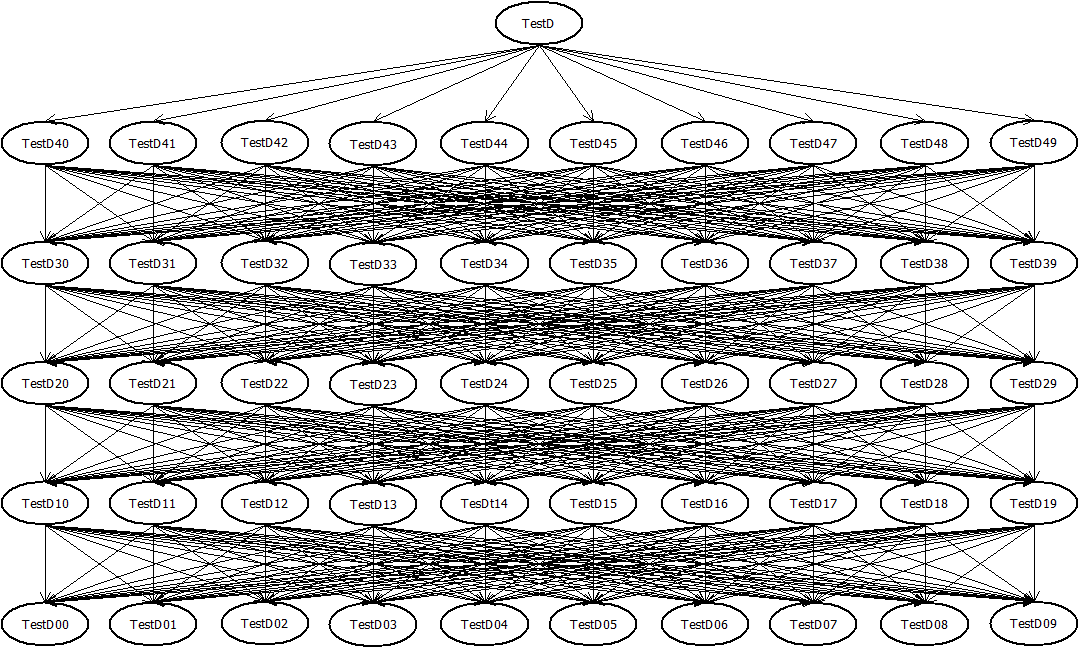
\includegraphics[width=\linewidth]{TestD.png}
  		\caption{Graf zależności dla testu D.}
  		\label{fig:testD}
	\end{center}
\end{figure}

Łatwo wywnioskować, że tworząc obiekty poszczególnych typów liczba tworzonych obiektów rośnie ponad dziesięciokrotnie:
\begin{itemize}
	\item typy od TestD00 do TestD09 - 1 obiekt,
	\item typy od TestD10 do TestD19 - 11 obiektów (obiekt danego typu plus 10 obiektów typów od TestD00 do TestD09),
	\item typy od TestD20 do TestD29 - 111 obiektów (obiekt danego typu plus 10 obiektów typów od TestD10 do TestD19),
	\item typy od TestD30 do TestD39 - 1 111 obiektów,
	\item  typy od TestD40 do TestD49 - 11 111 obiektów,
	\item TestD - 111 111 obiektów.
\end{itemize}
Zatem tworząc obiekt typu TestD, tworzymy: 1 obiekt typu TestD, 10 obiektów typów od TestD40 do TestD49, 100 obiektów typów od TestD30 do TestD39, 1 000 obiektów typów od TestD20 do TestD29, 10 000 obiektów typów od TestD10 do TestD19, 100 000 obiektów typów od TestD00 do TestD09 - co daje w sumie 111 111 obiektów.

\subsubsection{Wyniki Resolve dla Singleton}
\begin{table}[H]
\captionsetup{belowskip=0pt,aboveskip=0pt}
\begin{center}
\begin{small}
	\begin{tabular}{ | l | r r r | }
    		\hline
Liczba & & 1 & \\ \hline
 & min & max & avg \\ \hline
Autofac & 0 & 0 & 0 \\ \hline
Windsor & 0 & 0 & 0 \\ \hline
NiquIoCPartial & 8 & 9 & 9 \\ \hline
DryIoc & 10 & 10 & 10 \\ \hline
SimpleInjector & 11 & 12 & 11 \\ \hline
LightInject & 14 & 14 & 14 \\ \hline
Grace & 16 & 17 & 16 \\ \hline
NiquIoCFull & 18 & 19 & 18 \\ \hline
Ninject & 21 & 22 & 21 \\ \hline
StructureMap & 49 & 50 & 49 \\ \hline
Unity & 52 & 53 & 52 \\ \hline
  	\end{tabular}
\end{small}
\end{center}
\caption{Wyniki testów dla 1 powtórzenia dla operacji Singleton dla Przypadku testowego D}
\label{TestCaseD_Singleton1}
\end{table}
Dla tego testu tabela z wynikami bardzo przypomina tabelę dla przypadku testowego C, jednakże czasy są około 2-3 razy większe. Po raz kolejny dla rejestracji Singleton najlepiej radzą sobie Autofac i Windsor, a najsłabiej StructureMap i Unity.
\\ \\
\begin{table}[H]
\captionsetup{belowskip=0pt,aboveskip=0pt}
\begin{center}
\begin{small}
	\begin{tabular}{ | l | r r r | }
    		\hline
Liczba & & 10 & \\ \hline
 & min & max & avg \\ \hline
Autofac & 0 & 0 & 0 \\ \hline
Windsor & 0 & 0 & 0 \\ \hline
NiquIoCPartial & 8 & 9 & 8 \\ \hline
DryIoc & 10 & 10 & 10 \\ \hline
SimpleInjector & 11 & 12 & 11 \\ \hline
LightInject & 14 & 15 & 14 \\ \hline
Grace & 16 & 17 & 16 \\ \hline
NiquIoCFull & 18 & 19 & 18 \\ \hline
Ninject & 21 & 22 & 21 \\ \hline
StructureMap & 49 & 50 & 49 \\ \hline
Unity & 52 & 54 & 52 \\ \hline
  	\end{tabular}
\end{small}
\end{center}
\caption{Wyniki testów dla 10 powtórzeń dla operacji Singleton dla Przypadku testowego D}
\label{TestCaseD_Singleton10}
\end{table}
Jak można się było spodziewać, tym razem również wzrost liczby powtórzeń nie miał wpływu na wzrost wyników.

\subsubsection{Wyniki Resolve dla Transient}
\begin{table}[H]
\captionsetup{belowskip=0pt,aboveskip=0pt}
\begin{center}
\begin{small}
	\begin{tabular}{ | l | r r r | }
    		\hline
Liczba & & 1 & \\ \hline
 & min & max & avg \\ \hline
NiquIoCPartial & 36 & 38 & 37 \\ \hline
StructureMap & 102 & 110 & 103 \\ \hline
Autofac & 136 & 160 & 147 \\ \hline
Unity & 150 & 200 & 152 \\ \hline
SimpleInjector & 177 & 179 & 178 \\ \hline
Windsor & 177 & 261 & 182 \\ \hline
NiquIoCFull & 566 & 576 & 569 \\ \hline
LightInject & 797 & 831 & 812 \\ \hline
DryIoc & 979 & 996 & 982 \\ \hline
Ninject & 1016 & 1179 & 1039 \\ \hline
Grace & 1413 & 1472 & 1426 \\ \hline
  	\end{tabular}
\end{small}
\end{center}
\caption{Wyniki testów dla 1 powtórzenia dla operacji Transient dla Przypadku testowego D}
\label{TestCaseD_Transient1}
\end{table}
Test dla tego przypadku testowego pokazał dużo większe różnice czasów niż dla poprzednich przypadków testowych. Dla 1 powtórzenia wyraźniej najlepszy czas zanotował NiquIoCPartial, który osiągnął czas o rząd wielkości niższy niż kolejne rozwiązanie. Średnie czasy zanotowały StructureMap, Autofac, Unity oraz Windsor. Pozostałe rozwiązania razem z NiquIoCFull osiągnęły  bardzo duże wyniki.
\\ \\
\begin{table}[H]
\captionsetup{belowskip=0pt,aboveskip=0pt}
\begin{center}
\begin{small}
	\begin{tabular}{ | l | r r r | }
    		\hline
Liczba & & 10 & \\ \hline
 & min & max & avg \\ \hline
SimpleInjector & 205 & 212 & 206 \\ \hline
NiquIoCPartial & 285 & 291 & 287 \\ \hline
StructureMap & 586 & 603 & 591 \\ \hline
NiquIoCFull & 619 & 661 & 631 \\ \hline
LightInject & 841 & 878 & 853 \\ \hline
DryIoc & 1013 & 1025 & 1015 \\ \hline
Unity & 1073 & 1183 & 1080 \\ \hline
Autofac & 1161 & 1279 & 1188 \\ \hline
Grace & 1465 & 1558 & 1495 \\ \hline
Windsor & 1797 & 2421 & 1827 \\ \hline
Ninject & 10072 & 11599 & 10307 \\ \hline
  	\end{tabular}
\end{small}
\end{center}
\caption{Wyniki testów dla 10 powtórzeń dla operacji Transient dla Przypadku testowego D}
\label{TestCaseD_Transient10}
\end{table}
Wzrost liczby powtórzeń do 10 pokazał, że zarówno NiquIoCFull jak i prawie wszystkie najszybsze rozwiązania zanotowały niewielki wzrost. Wyjątkiem jest tutaj DryIoC, który osiągnął 10-krotny przyrost czasu. Jednakże bardzo duże wyniki już dla 1 powtórzenia spowodowały, że z najszybszy rozwiązań jedynie SimpleInjector ma nieduży czas. NiquIoCPartial pomimo 9-krotnego wzrostu czasu osiągnął drugi z najlepszych wyników. Wszystkie najpopularniejsze rozwiązania zanotowały wzrost około 10-krotny.

\subsubsection{Wyniki Resolve dla TransientSingleton}
\begin{table}[H]
\captionsetup{belowskip=0pt,aboveskip=0pt}
\begin{center}
\begin{small}
	\begin{tabular}{ | l | r r r | }
    		\hline
Liczba & & 1 & \\ \hline
 & min & max & avg \\ \hline
NiquIoCPartial & 17 & 18 & 17 \\ \hline
StructureMap & 60 & 69 & 61 \\ \hline
Autofac & 77 & 84 & 78 \\ \hline
SimpleInjector & 85 & 87 & 86 \\ \hline
Windsor & 85 & 102 & 87 \\ \hline
Unity & 115 & 140 & 116 \\ \hline
NiquIoCFull & 144 & 151 & 145 \\ \hline
Grace & 374 & 386 & 376 \\ \hline
Ninject & 503 & 572 & 511 \\ \hline
DryIoc & 905 & 922 & 910 \\ \hline
LightInject & 1285 & 1358 & 1310 \\ \hline
  	\end{tabular}
\end{small}
\end{center}
\caption{Wyniki testów dla 1 powtórzenia dla operacji TransientSingleton dla Przypadku testowego D}
\label{TestCaseD_TransientSingleton}
\end{table}
Dla tego testu ponownie dla 1 powtórzenia najmniejszy czas osiągnął NiquIoCPartial. Z pozostałych rozwiązań, to jedynie Grace, Ninject, DryIoC i LightInject zanotowały bardzo duże wyniki.
\\ \\
\begin{table}[H]
\captionsetup{belowskip=0pt,aboveskip=0pt}
\begin{center}
\begin{small}
	\begin{tabular}{ | l | r r r | }
    		\hline
Liczba & & 10 & \\ \hline
 & min & max & avg \\ \hline
SimpleInjector & 91 & 93 & 91 \\ \hline
NiquIoCPartial & 100 & 104 & 101 \\ \hline
NiquIoCFull & 151 & 159 & 152 \\ \hline
StructureMap & 165 & 173 & 167 \\ \hline
Grace & 381 & 396 & 383 \\ \hline
Unity & 683 & 771 & 689 \\ \hline
Windsor & 852 & 965 & 864 \\ \hline
Autofac & 893 & 964 & 910 \\ \hline
DryIoc & 936 & 983 & 942 \\ \hline
LightInject & 1297 & 1360 & 1316 \\ \hline
Ninject & 4732 & 5620 & 4818 \\ \hline
  	\end{tabular}
\end{small}
\end{center}
\caption{Wyniki testów dla 10 powtórzeń dla operacji TransientSingleton dla Przypadku testowego D}
\label{TestCaseD_TransientSingleton10}
\end{table}
Gdy liczba operacji wzrosła do 10, to jak można się było spodziewać - NiquIoCPartial zanotował około 5-krotny wzrost, a najpopularniejsze rozwiązania zanotowały około 10-krotny wzrost. NiquIoCFull oraz najszybsze rozwiązania osiągnęły czasy zbliżone do czasów dla 1 powtórzenia. Najmniejszy czas uzyskał SimpleInjector, a trochę większe rezultaty zanotowały NiquIoCPartial, NiquIoCFull i StructureMap. Pozostałe rozwiązania osiągnęły zauważalnie większe czasy - od kilku do nawet kilkunastu razy.

\subsubsection{Wyniki Resolve dla PerThread}
\begin{table}[H]
\captionsetup{belowskip=0pt,aboveskip=0pt}
\begin{center}
\begin{small}
	\begin{tabular}{ | l | r r r | }
    		\hline
Liczba & & 1 & \\ \hline
 & min & max & avg \\ \hline
Autofac & 0 & 0 & 0 \\ \hline
Windsor & 0 & 0 & 0 \\ \hline
NiquIoCPartial & 8 & 9 & 9 \\ \hline
NiquIoCFull & 18 & 18 & 18 \\ \hline
Ninject & 21 & 22 & 21 \\ \hline
Grace & 28 & 28 & 28 \\ \hline
SimpleInjector & 46 & 48 & 46 \\ \hline
StructureMap & 49 & 51 & 49 \\ \hline
Unity & 52 & 53 & 52 \\ \hline
DryIoc & 1042 & 1051 & 1045 \\ \hline
LightInject & 762748 & 795038 & 773697 \\ \hline
  	\end{tabular}
\end{small}
\end{center}
\caption{Wyniki testów dla 1 powtórzenia dla operacji PerThread dla Przypadku testowego D}
\label{TestCaseD_PerThread1}
\end{table}
Wyniki dla tego testu są podobne jak w pozostałych przypadkach testowych. Jedynym wyjątkiem jest LightInject, który najwyraźniej nie poradził sobie z tak dużo liczbą obiektów dla tego typu rejestracji i zanotował czas o 5 rzędów wielkości większy, niż rozwiązania z najmniejszymi czasami - Autofac, Windsor i NiquIoCPartial.
\\ \\
\begin{table}[H]
\captionsetup{belowskip=0pt,aboveskip=0pt}
\begin{center}
\begin{small}
	\begin{tabular}{ | l | r r r | }
    		\hline
Liczba & & 10 & \\ \hline
 & min & max & avg \\ \hline
Autofac & 0 & 0 & 0 \\ \hline
Windsor & 0 & 0 & 0 \\ \hline
NiquIoCPartial & 8 & 10 & 9 \\ \hline
NiquIoCFull & 18 & 18 & 18 \\ \hline
Ninject & 21 & 22 & 21 \\ \hline
Grace & 28 & 28 & 28 \\ \hline
SimpleInjector & 46 & 48 & 46 \\ \hline
StructureMap & 49 & 51 & 49 \\ \hline
Unity & 52 & 53 & 52 \\ \hline
DryIoc & 1042 & 1051 & 1044 \\ \hline
LightInject & 763101 & 781163 & 774677 \\ \hline
  	\end{tabular}
\end{small}
\end{center}
\caption{Wyniki testów dla 10 powtórzeń dla operacji PerThread dla Przypadku testowego D}
\label{TestCaseB_PerThread10}
\end{table}
Przy 10 powtórzeniach nic się nie zmieniło i wyniki są zbliżone do wyników dla 1 powtórzenia.

\subsubsection{Wyniki Resolve dla FactoryMethod}
\begin{table}[H]
\captionsetup{belowskip=0pt,aboveskip=0pt}
\begin{center}
\begin{small}
	\begin{tabular}{ | l | r r r | }
    		\hline
Liczba & & 1 & \\ \hline
 & min & max & avg \\ \hline
DryIoc & 9 & 10 & 10 \\ \hline
LightInject & 12 & 13 & 12 \\ \hline
NiquIoCPartial & 15 & 17 & 15 \\ \hline
SimpleInjector & 20 & 20 & 20 \\ \hline
NiquIoCFull & 20 & 21 & 20 \\ \hline
Grace & 24 & 25 & 24 \\ \hline
Autofac & 67 & 80 & 68 \\ \hline
StructureMap & 90 & 93 & 91 \\ \hline
Windsor & 127 & 136 & 129 \\ \hline
Unity & 173 & 181 & 174 \\ \hline
Ninject & 654 & 748 & 674 \\ \hline
  	\end{tabular}
\end{small}
\end{center}
\caption{Wyniki testów dla 1 powtórzenia dla operacji FactoryMethod dla Przypadku testowego D}
\label{TestCaseB_FactoryMethod1}
\end{table}
NiquIoCPartial, NiquIoCFull oraz wszystkie najszybsze rozwiązania zanotowały zbliżone wyniki. Rozwiązania najpopularniejsze osiągnęły czasy od kilku, do kilkunastu razy większe. Najlepszy czas uzyskał DryIoC.
\\ \\
\begin{table}[H]
\captionsetup{belowskip=0pt,aboveskip=0pt}
\begin{center}
\begin{small}
	\begin{tabular}{ | l | r r r | }
    		\hline
Liczba & & 10 & \\ \hline
 & min & max & avg \\ \hline
DryIoc & 78 & 81 & 79 \\ \hline
LightInject & 79 & 83 & 80 \\ \hline
SimpleInjector & 128 & 131 & 129 \\ \hline
Grace & 127 & 149 & 130 \\ \hline
NiquIoCPartial & 164 & 170 & 166 \\ \hline
NiquIoCFull & 185 & 191 & 188 \\ \hline
StructureMap & 592 & 610 & 597 \\ \hline
Autofac & 671 & 799 & 685 \\ \hline
Windsor & 1227 & 1284 & 1238 \\ \hline
Unity & 1744 & 1839 & 1769 \\ \hline
Ninject & 6206 & 6515 & 6299 \\ \hline
  	\end{tabular}
\end{small}
\end{center}
\caption{Wyniki testów dla 10 powtórzeń dla operacji FactoryMethod dla Przypadku testowego D}
\label{TestCaseB_FactoryMethod10}
\end{table}
Wzrost liczby powtórzeń do 10 spowodował wzrost czasów dla wszystkich rozwiązań. Najmniejszy wzrost czasów zanotowały najszybsze rozwiązania, jednak wciąż był on co najmniej 6-krotny. NiquIoCPartial i NiquIoCFull podobnie jak wszystkie najpopularniejsze rozwiązania zanotowały wzrost około 10-krotny. Jednakże nieduże czasy przy 1 powtórzeniu dla rozwiązań zaprezentowanych w tej pracy spowodowały, że mimo wszystko osiągnęły one znacząco lepsze wyniki niż wszystkie najpopularniejsze rozwiązania. Najlepsze czasy uzyskały wszystkie najszybsze rozwiązania, a najmniejsze z tych czasów osiągnęły DryIoC i LightInject.



\clearpage
\section{Podsumowanie}
Zaproponowane przeze mnie rozwiązania bardzo dobrze realizują postawione we wstępie pracy cele. Dla wszystkich przypadków testowych, dla każdego z rodzaju rejestracji jedno z moich rozwiązań radziło sobie najlepiej albo niewiele odbiegało od najlepszego rozwiązania (zawsze któreś z moich rozwiązało było w pierwszej trójce, a czasami nawet oba). Możliwość mieszania użyć zaprezentowanych przeze mnie rozwiązań (w jednym projekcie można korzystać z obu rozwiązań niezależnie) sprawia, że NiquIoC jest najwydajniejszą implementacją wzorca wstrzykiwania zależności dla złożonych grafów zależności.\\ 
\\
Dodatkowo wyniki moich testów pokazują, że rozwiązanie Ninject jest najmniej wydajne i nie zaleca się go używać przy bardzo rozbudowanych grafach. Jeśli chodzi natomiast o rozwiązania, które radzą sobie dobrze, to nie ma drugiego takiego (poza moim), które zawsze dawałoby zadowalające rezultaty. SimpleInjector dość dobrze radzi sobie dla testów Singleton, Transient i TransientSingleton, ale osiąga słabe rezultaty dla PerThread i FactoryMethod. LightInject z kolei jest rozwiązaniem, które wraz ze wzrostem liczby operacji ma najmniejszy wzrostu czasu. Jednakże w wielu przypadkach dość duże czasy dla małej liczby operacji powodują, że wyniki dla wielu operacji są bardzo duże. Takim pośrednim rozwiązaniem jest natomiast Grace. To rozwiązanie ma zarówno nieduże wzrosty czasów jak i nieduże wyniki dla małej ilości operacji, jednak mimo wszystko są one dużo słabsze niż dla NiquIoC.

\subsection{Kontynuacja projektu}
Zaprezentowane przeze mnie rozwiązania są bardzo wydaje, ale mają swoje ograniczenia. Jednym z nich jest między innymi konieczność rejestracji wszystkich typów. Tę funkcjonalność można by rozszerzyć, aby nie trzeba było rejestrować klas. Algorytm sam rejestrowałby klasy, gdyby okazywały się potrzebne - większość z rozwiązań dostarcza taką funkcjonalność. Kolejnym rozszerzeniem mogłoby być automatyczna rejestracja wszystkich typów z danego assembly. Osobom wykorzystującym moje rozwiązanie zaoszczędziłoby to sporo czasu na rejestrowanie wszystkich typów. Dodatkowo dodając kolejny typ do danego assembly, nie trzeba byłoby się przejmować zarejestrowaniem go. Jeszcze jednym dodatkiem wydaje się danie możliwości rejestracji wielu implementacji danego interfejsu. To jest również często spotykana funkcjonalność. Na koniec warto również wspomnieć o metodzie BuildUp dla NiquIoCFull - w mojej pracy tego zabrakło, a to również mogłoby być jednym z kolejnych rozszerzeń.

\newpage
\listoffigures
\listoftables

\newpage
\begin{thebibliography}{authordate1}
\bibitem{csharp} Ian Griffiths, Matthew Adams, Jesse Liberty, C\#. Programowanie. Wydanie VI, 2012
\bibitem{dependency_injection} Mark Seemann, Dependency Injection in .NET, 2012
\bibitem{emit} Serge Lidin, Expert .NET 2.0 IL Assembler, 2006
\bibitem{clean_code} Robert C. Martin, Czysty kod. Podręcznik dobrego programisty, 2014
\bibitem{SOLID} https://en.wikipedia.org/wiki/SOLID\_(object-oriented\_design)
\end{thebibliography}

\end{document}